\documentclass[
    reprint, 
    aps,
    preprintnumbers,
    twocolumn,
    prb,
    superscriptaddress
]{revtex4-2}


%=======================
% Packages:
%=======================

\usepackage[utf8]{inputenc}
\usepackage{booktabs}
\usepackage[multiple]{footmisc}
\usepackage{lipsum}
\usepackage{rotating}
\usepackage{perpage}
\usepackage{chronology}
\usepackage{amssymb}
\usepackage{amsbsy}
\usepackage{amsmath}
\usepackage{tikz}
\usepackage[T1]{fontenc}
\usepackage{etoolbox}
\usepackage{graphics}
\usepackage{abraces}
\makeatletter
\let\unit\relax % otherwise there are package conflicts with siunitx
\makeatother
\usepackage{siunitx}
\usepackage{hyperref}
%\usepackage{float}
\usepackage{multirow}
\usepackage{mathtools}
\usepackage{bm}
\usepackage{url}
\usepackage{physics}
\usepackage{hyperref}
\usepackage{bbm}
\usepackage{color}
\usepackage{placeins}
\usepackage[normalem]{ulem}
%\usepackage{mhchem}

%=======================
% New Commands:
%=======================

\newcommand{\vk}{\vec{k}}
\newcommand{\vl}{\vec{l}}
\newcommand{\vQ}{\vec{Q}}
\newcommand{\up}{\uparrow}
\newcommand{\down}{\downarrow}
\newcommand{\kplusQ}{\vk+\vQ}
\newcommand{\kminusQ}{-\vk-\vQ}
\newcommand{\im}{\mathrm{i}}

\newcommand{\ddt}{\frac{\mathrm{d}}{\mathrm{d}t}}
\newcommand{\dgamma}{\mathrm{d}\gamma}

\newcommand{\mM}{\mathcal{M}}
\newcommand{\mN}{\mathcal{N}}

\newcommand{\greens}[1]{\mathcal{G}_\text{#1} (\omega)}
\newcommand{\green}[1]{\mathcal{G}_\text{#1}}
\newcommand{\spectral}[1]{\mathcal{A}_\text{#1}  (\omega)}

\newcommand{\markEdited}{red}

\newcommand{\bs}{\begin{subequations}}
\newcommand{\es}{\end{subequations}}
\newcommand{\be}{\begin{equation}}
\newcommand{\ee}{\end{equation}}

\newcommand{\red}[1]{\textcolor{red}{#1}}
\newcommand{\blue}[1]{\textcolor{blue}{#1}}

\def\hmath$#1${\texorpdfstring{{\rmfamily\textit{#1}}}{#1}}

\begin{document} 

% Preliminary title
\title{Collective excitations in competing phases in two and three dimensions}

%=======================
% Authors:
%=======================

\author{Joshua Alth\"user}\email{joshua.althueser@tu-dortmund.de}
\affiliation{Condensed Matter Theory, TU Dortmund University,
Otto-Hahn Stra\ss{}e 4, 44227 Dortmund, Germany}

\author{G\"otz S.~Uhrig}
\email{goetz.uhrig@tu-dortmund.de}
\affiliation{Condensed Matter Theory, TU Dortmund University,
Otto-Hahn Stra\ss{}e 4, 44227 Dortmund, Germany}

\date{\today}

%%%%%%%%%%%%%%%%%%%%%%%%%%%%%%%%%%%%%%%%%%%%%%%%%%%%%%%%%%%%%%%%%%%%%%%%%%%%%%%%%%%%%%%%%%%%%%%%%%%%%%%%%%%%%%%%%%%%%
%%%%%%%%%%%%%%%%%%%%%%%%%%%%%%%%%%%%%%%%%%%%%%%%%%%%%%%%%%%%%%%%%%%%%%%%%%%%%%%%%%%%%%%%%%%%%%%%%%%%%%%%%%%%%%%%%%%%%
%%%%%                                                  Abstract                                                 %%%%%
%%%%%%%%%%%%%%%%%%%%%%%%%%%%%%%%%%%%%%%%%%%%%%%%%%%%%%%%%%%%%%%%%%%%%%%%%%%%%%%%%%%%%%%%%%%%%%%%%%%%%%%%%%%%%%%%%%%%%
%%%%%%%%%%%%%%%%%%%%%%%%%%%%%%%%%%%%%%%%%%%%%%%%%%%%%%%%%%%%%%%%%%%%%%%%%%%%%%%%%%%%%%%%%%%%%%%%%%%%%%%%%%%%%%%%%%%%%
\begin{abstract}
    We investigate the superconducting (SC), charge-density wave (CDW), and antiferromagnetic (AFM) phases in the 
		extended Hubbard model at zero temperature and half-filling. 
    We employ the iterated equations of motion approach to compute the two-particle Green's functions and their
		spectral densities. 
    This renders a comprehensive analysis of the behavior of collective excitations possible as the 
		model's parameters are tuned across phase transitions. 
    We identify the well-known amplitude (Higgs) and phase (Anderson-Bogoliubov) modes within the 
		superconducting phase and observe a similar excitation (cooperon) in the CDW phase which shifts towards 
		zero energy as the system approaches the phase transition to the SC phase. 
    In the CDW phase, close to the phase transition to the AFM phase, 
    we find a collective mode, an exciton, that does not change significantly 
    and another mode, a longitudinal magnon, that emerges from the two-particle continuum as the system approaches the phase transition to the AFM phase. 
    \red{Habe ich geaendert - stimmt es so?} \blue{Nicht ganz, das Magnon verschwindet, wenn man weg von der Phasengrenze geht, also zu kleineren U/größeren V. 
    Umgekehrt in der AFM phase, verschwindet das Exziton, bei dem analogen Prozess, also zu großem U/kleinen V. Des Weiteren sind beide Magnonen außerhalb der AFM Phase identisch.
    Ist es dann richtig, hier nur von dem longitudinalen zu sprechen?}
		In the AFM phase, we identify both a longitudinal (amplitude) and a 
		transversal Goldstone magnon; the latter is located at zero energy.
\end{abstract}

\maketitle

%%%%%%%%%%%%%%%%%%%%%%%%%%%%%%%%%%%%%%%%%%%%%%%%%%%%%%%%%%%%%%%%%%%%%%%%%%%%%%%%%%%%%%%%%%%%%%%%%%%%%%%%%%%%%%%%%%%%%
%%%%%%%%%%%%%%%%%%%%%%%%%%%%%%%%%%%%%%%%%%%%%%%%%%%%%%%%%%%%%%%%%%%%%%%%%%%%%%%%%%%%%%%%%%%%%%%%%%%%%%%%%%%%%%%%%%%%%
%%%%%                                                Introduction                                               %%%%%
%%%%%%%%%%%%%%%%%%%%%%%%%%%%%%%%%%%%%%%%%%%%%%%%%%%%%%%%%%%%%%%%%%%%%%%%%%%%%%%%%%%%%%%%%%%%%%%%%%%%%%%%%%%%%%%%%%%%%
%%%%%%%%%%%%%%%%%%%%%%%%%%%%%%%%%%%%%%%%%%%%%%%%%%%%%%%%%%%%%%%%%%%%%%%%%%%%%%%%%%%%%%%%%%%%%%%%%%%%%%%%%%%%%%%%%%%%%

\section{Introduction}\label{sec:introduction}


The study of collective excitations is of great interest as it sheds light on the intricate dynamics of correlated electron systems, providing crucial insight into emergent material properties.
We are in particular interested in the behavior of the collective excitations in the vicinity of phase transitions.
Do they signal these transitions, for instance by softening? 
How does the competition of different phases manifest in the energies and weights of the collective excitations?
These questions set the context of the present article. 

On the theoretical side, we choose a paradigmatic, but simple model which displays competing phases.
The Hubbard model has been employed in a plethora of previous studies and competing phases are established in its extensions. 
Early studies proved the existence of eigenstates of the Hubbard Hamiltonian that exhibit off-diagonal long-range order, encouraging the model's usage for the description of high-temperature superconductivity \cite{yang89}.
Shortly afterward, an exact SO(4) symmetry was discovered, which induces a degeneracy of 
superconductivity (SC) and a charge-density wave (CDW) governed by an attractive on-site interaction \cite{yang90}.
This coexistence stems from the existence of a particle-hole transformation on bipartite lattices, 
that maps the attractive Hubbard model rigorously onto the repulsive one, 
exhibiting antiferromagnetism (AFM) \cite{Hirsch85}.
The order parameters of the previously mentioned SC and CDW phases map to different spin expectation values \cite{zitko15,lieb89}.
\blue{Den vorigen Satz verstehe ich leider gar nicht: phase = spin operator? Ja, das war ungenau. So ist es vermutlich besser?}

Numerous studies investigated the phases and various quantities of the Hubbard model in equilibrium systems, including additional interactions with and without doping
\cite{Micnas88,Micnas88b,Micnas89,Dzierzawa92,Kostyrko92,Eriksson95,Staudt00,Onari04,Toschi05,Brackett16,Paki19,romer20,Sushchyev22}. 
Recent studies on the dynamics of the superconducting gap parameter examined quenches, yielding oscillations \cite{Volkov73,Yuzbashyan05,Yuzbashyan06,Barankov06,Cui19}, 
and driven systems motivated by the goal to induce superconductivity \cite{Nicoletti14,Krull14,Moor14,Casandruc15,patel16,sentef17,Buenemann17}.

In this paper, we restrict ourselves to the half-filled Hubbard model 
including an additional nearest neighbor, intersite interaction on the square and the simple cubic lattice at zero temperature.
Specifically, we investigate competing phases, i.e., the behavior of various collective modes close to phase transitions between these phases.
To this end, the case in two dimensions (2D) already displays a wide range of possible phases
including CDW, AFM, $s$- and $d_{x^2 - y^2}$-wave superconductivity as well as 
phase-separated states \cite{Micnas88b,Tsuchiura95,Su01,Su04,ha11,Huang13,Jiang22,Linner23}.
We extend the corresponding established phase diagrams to the simple cubic lattice in three dimensions
(3D) where we find a qualitatively similar phase diagran for CDW, AFM, $s$-wave SC phases, and
indications of phase separation.

First, we employ a mean-field approximation to the interaction terms to determine the phases.
Second, we use the iterated equations of motion approach (iEoM)
which has already seen success in the handling of interaction quenches \cite{uhrig09,hamerla13,hamerla14,bleicker18}
to compute the collective excitations.
The basic idea is to start in the Heisenberg picture from a suitable operator basis which is extended
upon commuting its operators with the Hamiltonian and including the appearing additional operators to the basis. 
Of course, a truncation is necessary for most practical applications, however, the approximation becomes better the more terms are included within the basis.
The applicability of this method was compared successfully to the results of the density matrix formalism \cite{Kalthoff17}.

Moreover, we demonstrate an explicit way to compute various Green's functions by this approach.
By extension, the corresponding spectral functions of the investigated systems can be computed and 
we discuss the signatures of collective excitations in the spectral functions. \blue{within these?}
The most prominent examples in the SC phase are the well-known phase mode (Anderson-Bogoliubov) and 
the amplitude (Higgs) modes. The former occurs in neutral superfluids at zero energy and was found
in a large number of studies \cite{Bogoljubov1958,Anderson58,Brieskorn74,Schmid1975,simanek1975,schon76,Maiti2015,Sun2020,Fan22} which we cannot list exhaustively here.
We obtain this mode based on a microscopic description without long-range electromagnetic interactions.
The inclusion of this kind of interaction would shift this mode towards the plasma frequency 
\cite{Anderson58,schon76,Kulik1981} which is, however, beyond the scope of the present paper. 
The amplitude mode, on the other hand, is located at the lower edge of the quasiparticle continuum.
The corresponding energy is the energy required to break up a Cooper pair 
\cite{Schmid1975,Varma02,Cea14,Measson14,Tsuji15,Krull16,Mueller2019,Schwarz20}.
This Higgs mode is not charged so that it does not couple to the electromagnetic fields.

This paper is organized as follows:
In \autoref{sec:model} we introduce the model and its Hamiltonian as well as the employed mean-field theory for the ground state.
We give a brief overview of the iterated equations of motion approach and 
derive a rigorous relation to Green's functions in \autoref{sec:ieom}.
Next, we show and discuss results in \autoref{sec:results}.
Lastly, in \autoref{sec:conclusion}, we summarize the results, draw the conclusions, and provide
an outlook.

\section{Model and mean-field theory}\label{sec:model}

\subsection{Model}

In our study, we employ the extended Hubbard model at half-filling as it hosts
the relevant phases and thereby provides direct access to the rich excitation spectra therein.
Its Hamiltonian is given by
\begin{align}
\nonumber
        H = &-t \sum_{\langle i, j \rangle, \sigma} \left( c_{i\sigma}^\dagger c_{j\sigma} + \text{h.c.} \right) 
        + \mu \sum_{i,\sigma} n_{i\sigma} \\
        & + U \sum_{i} n_{i\uparrow} n_{i\downarrow} 
        + \frac{V}{2} \sum_{\langle i, j\rangle, \sigma} n_{i\sigma} n_{j\sigma},
				    \label{eqn:full_hamiltonian}
\end{align}
where $c_{i\sigma}^{(\dagger)}$ annihilates (creates) an electron with spin $\sigma$ on lattice site $i$ 
and $\langle i, j\rangle$ denotes the summation over nearest neighbor sites.
The parameters are the hopping amplitude $t$, the onsite interaction $U$, the intersite interaction $V$, and the chemical potential $\mu$.
Applying a Fourier transform passing to $k$ space yields the single-particle dispersion 
\begin{equation}
    \epsilon_0 (\vk) = -2t \sum_{\alpha=1}^D \cos(k_\alpha), \quad k_\alpha \in [-\pi, \pi)\,,
\end{equation}
with the system's dimension $D$ and the dimensionless wave vector $\vk$ where we set the lattice constant to unity.

We investigate this model for various sets of parameters allowing us access to a variety of phases.
The model exhibits antiferromagnetism for positive $U$ and moderate values of $V$.
At larger $V$, the intersite repulsion takes over and favors a charge-ordered phase, i.e., a CDW.
In the $U<0$ region, the CDW occurs for any $V>0$.
Choosing $V=0$ leads to a coexistence of $s$-wave superconductivity and said CDW \cite{yang90}, while moderate
values of  $V<0$ yield an $s$-wave superconducting phase \cite{Micnas88b}.
In this article, we explore the AFM-CDW as well as the CDW-SC phase transitions.
For $U<0$ and $V<0$, signs of phase separation occur as one would expect.


\subsection{Static mean-field theory}

Next, we decouple the interaction terms according to Wick's theorem.
We define short hands for the operators
\bs
\begin{align}
    \label{eqn:operators}
        n_{k\sigma} &\coloneqq  c_{\vk\sigma}^\dagger c_{\vk\sigma}      &f_k     &\coloneqq  c_{-\vk\down} c_{\vk\up} \\
        g_{k\sigma} &\coloneqq  c_{\vk\sigma}^\dagger c_{\vk+\vQ\sigma}  &\eta_k  &\coloneqq  c_{-\vk-\vQ\down} c_{\vk\up}
\end{align}
\es
where $\vQ \coloneqq  (\pi, \pi)$ in 2D and $\vQ \coloneqq  (\pi, \pi,\pi)$ in 3D
defines the nesting vector for the CDW and AFM phases. We use the following abbreviations to write down the mean-field parameters
\begin{subequations}
    \begin{align}
        \label{eqn:delta_cdw}
        \Delta_\text{CDW} &= \left(\frac{U}{2N} - 
				\frac{zV}{N}\right) \sum_{\vk\sigma} \langle g_{\vk\sigma} \rangle \\
        \label{eqn:delta_afm}
        \Delta_\text{AFM} &= \frac{U}{2N} \sum_{\vk} \left( \langle g_{k\uparrow} \rangle - \langle g_{\vk\downarrow} \rangle \right), \\
        \Delta_\text{SC} &= \frac{U}{N} \sum_{\vk} \langle f_{\vk} \rangle, \\
        \Delta_\eta &= \frac{U}{N} \sum_{\vk} \langle \eta_{\vk} \rangle, \\
        \Delta_n &= \frac{V}{N} \sum_{\vk,\sigma} \sum_{\alpha=1}^D \cos k_\alpha \langle n_{\vk\sigma} \rangle,
    \end{align}
\end{subequations}
where $z$ denotes the coordination number of the lattice.
The last parameter, $\Delta_n$, renormalizes the hopping term according to 
\begin{equation}
    \epsilon( \vk ) \coloneqq  -(2 + \Delta_n) \sum_{\alpha=1}^D \cos(k_\alpha)\,.
\end{equation}
In total, we obtain the mean-field Hamiltonian in spinor representation as
\begin{equation}
    \label{eqn:mf_hamiltonian}
    H_\text{MF} = \sum_{\vk} \Psi^\dagger (\vk) h(\vk) \Psi (\vk)\,,
\end{equation}
with the spinors
\begin{equation}
    \Psi^\dagger (\vk) \coloneqq  \left( c_{\vk\up}^\dagger\,, c_{\kplusQ\up}^\dagger\,, c_{-\vk\down}\,, c_{\kminusQ\down} \right)
\end{equation}
and the matrix
\begin{equation}
    h(\vk) \coloneqq  \begin{pmatrix}
        \epsilon (\vk) & \Delta_-^* & \Delta_\text{SC} & \Delta_\eta \\
        \Delta_- & \epsilon (\vk + \vQ) & \Delta_\eta & \Delta_\text{SC} \\
        \Delta_\text{SC}^* & \Delta_\eta^* & - \epsilon (-\vk) & - \Delta_+ \\
        \Delta_\eta^* & \Delta_\text{SC}^* & - \Delta_+^* & - \epsilon (-\vk - \vQ)
        \end{pmatrix}\,,
\end{equation}
where we defined $\Delta_\pm \coloneqq \Delta_\text{CDW} \pm \Delta_\text{AFM}$.

\begin{figure}
    \centering
    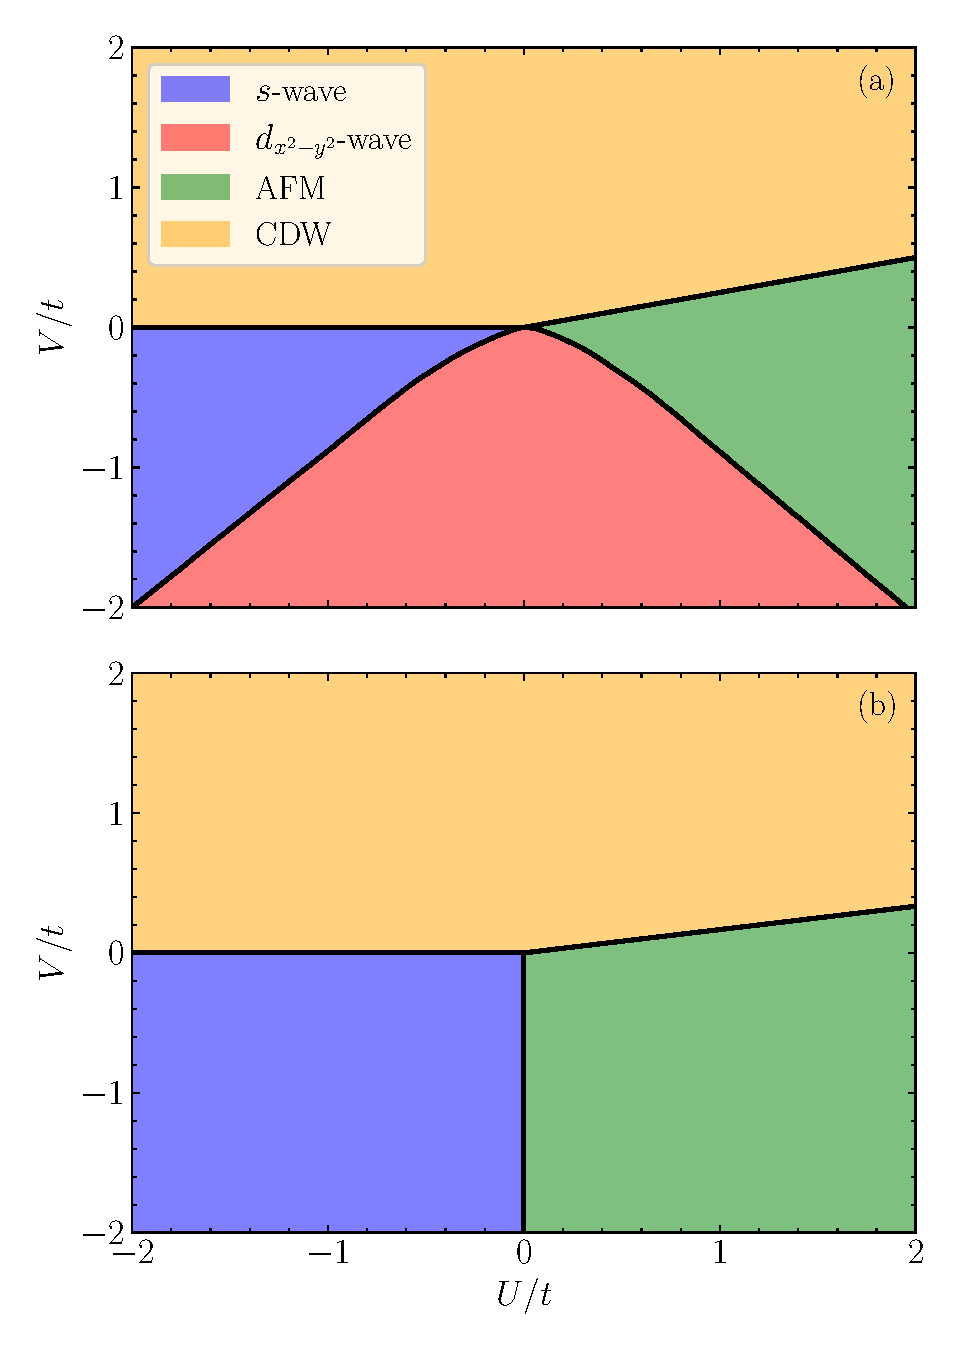
\includegraphics[width=.48\textwidth]{plots/phase_diagram.pdf}
    \caption{The phase diagram obtained for the extended Hubbard model \eqref{eqn:full_hamiltonian} on 
    (a) a square lattice and (b) a simple cubic lattice using a mean-field approximation at $T=0$.
    The CDW-AFM boundary lies at $U = zV$, where $z$ is the coordination number. 
    For $U<0$ and $V=0$,  CDW and $s$-wave SC coexist.
    The boundary for the $d_{x^2 - y^2}$-wave SC (dashed line) for the square lattice is  taken from Ref.\
		\cite{Micnas88b} since it is not accessible within our formalism, see below.
    However, the red shading indicates the region in which the dynamical matrix $\mM$ in 
		Eq.\ \eqref{eqn:heisenberg}, has negative eigenvalues indicating the instability of the assumed phase.
    In view of the attractive interactions, we expect a separation of phases \cite{Linner23}.
    Lastly, the striped area shows the region that we cannot access numerically
		because the gap values are too small for any tractable discretization. 
    Yet an SC phase is expected.}
    \label{fig:phase_diagram}
\end{figure}

We observe that  the entire Hamiltonian and all expectation values in the considered phases only depend on
\begin{equation}
    \widehat{\gamma}(\vk) \coloneqq \frac{1}{D} \sum_{\alpha=1}^D \cos(k_\alpha),
\end{equation}
i.e., for any operator $\widehat{O}$ the following relation holds 
\begin{equation}
    \label{eqn:equal_expecs}
    \langle \widehat{O}_{\vk} \rangle = \langle \widehat{O}_{\vk'} \rangle \eqqcolon \langle \widehat{O}( \gamma ) \rangle\,,
\end{equation}
if $\gamma= \widehat{\gamma}(\vk) = \widehat{\gamma}(\vk')$.
While 2D systems  of about $100\times100$ lattice sites can still be solved by evaluating sums over  wave vectors,
computing solutions for large three-dimensional systems becomes impossible due to the $N=L^3$ scaling.
This issue can be resolved by using the aforementioned fact and replacing the wave vector sums 
by energy integrals using the density of states (DOS) for $\gamma$ defined by
\begin{equation}
    \rho(\gamma) \coloneqq  \frac{1}{N} \sum_{\vk} \delta \left(\gamma - \widehat{\gamma} (\vk) \right)\,.
\end{equation}
As an example, we consider 
\begin{equation}
    \Delta_\text{SC} = \frac{U}{N} \int_{-1}^{1} \dgamma \rho(\gamma) \langle f( \gamma ) \rangle\,.
\end{equation}
Henceforth, we use the exact DOS for the square and the simple cubic lattice provided 
in Ref.\ \cite{Hanisch97}. 
This allows us to access both 2D and 3D models on equal footing.
We can compute any phase as long as it does not introduce another kind of wave vector dependence.


We solve the mean-field equations self-consistently.
The $\gamma$ integrals are approximated numerically using a $\tanh$-$\sinh$ quadrature \cite{takahasi73} 
terminating once $|1 - \int \dgamma \rho(\gamma)| < 10^{-13}$ is achieved
and reusing the computed sampling points and weights.
This method excels at dealing with the singularities in the DOS 
requiring merely a few hundred function evaluations to achieve the desired accuracy.

This procedure yields the ground state phase diagram at $T=0$ shown in Fig.\ 
\ref{fig:phase_diagram}.
The CDW-AFM boundary is located at $U = zV$, where $z$ is the coordination number.
This holds for both the square lattice ($z=4$) and the simple cubic lattice ($z=6$) and can be seen by comparing the prefactors in Eqs.\ \eqref{eqn:delta_cdw} and \eqref{eqn:delta_afm}:
Crossing $U = zV$ changes which prefactor of the two order parameters is larger.

Note, that the $d_{x^2 - y^2}$-superconducting state, which has been confirmed for the square lattice 
\cite{Micnas88b,Huang13}, cannot be described by our method because it would require to 
deal with expectations values which do not depend only on $\widehat{\gamma}(\vk)$.

%%%%%%%%%%%%%%%%%%%%%%%%%%%%%%%%%%%%%%%%%%%%%%%%%%%%%%%%%%%%%%%%%%%%%%%%%%%%%%%%%%%%%%%%%%%%%%%%%%%%%%%%%%%%%%%%%%%%%
%%%%%%%%%%%%%%%%%%%%%%%%%%%%%%%%%%%%%%%%%%%%%%%%%%%%%%%%%%%%%%%%%%%%%%%%%%%%%%%%%%%%%%%%%%%%%%%%%%%%%%%%%%%%%%%%%%%%%
%%%%%                                                  Methods                                                  %%%%%
%%%%%%%%%%%%%%%%%%%%%%%%%%%%%%%%%%%%%%%%%%%%%%%%%%%%%%%%%%%%%%%%%%%%%%%%%%%%%%%%%%%%%%%%%%%%%%%%%%%%%%%%%%%%%%%%%%%%%
%%%%%%%%%%%%%%%%%%%%%%%%%%%%%%%%%%%%%%%%%%%%%%%%%%%%%%%%%%%%%%%%%%%%%%%%%%%%%%%%%%%%%%%%%%%%%%%%%%%%%%%%%%%%%%%%%%%%%

\section{Iterated equations of motion and Green's functions}
\label{sec:ieom}

So far we discussed the static mean-field equations that describe the ground state.
These results are used to compute the quantities, namely the expectation values, necessary for the iterated equations of motion approach \cite{uhrig09,hamerla13,hamerla14,bleicker18}.
On this basis, we can describe two-particle quantities such as the various collective excitations of the system.

We start with an operator set $\mathcal{B}$ that ideally is complete with respect to commutation with 
the Hamiltonian $H$, i.e., any commutator $[H, A]$ for any $A \in \mathcal{B}$ can be represented by linear combinations of operators in $\mathcal{B}$.
Then, we can express any time-dependent operator in this set by
\begin{equation}
    \label{eqn:time_dependent_operator}
    A(t) = \sum_n a_n(t) A_n,
\end{equation}
where the coefficients $c_j(t)$ capture the entire time dependence. 
Inserting this into the Heisenberg equation of motion and applying a sort of operator scalar product $(A_i|\cdot)$ 
on both sides of the equation yields
\bs
\begin{align}
        \ddt A(t) = \sum_n \ddt a_n(t) A_n &= \im \sum_n a_n(t) [H, A_n] \\
        \Rightarrow \sum_n \underbrace{(A_i | A_n)}_{\coloneqq \mN_{in}} \ddt a_n(t) &= 
				\im \sum_n \underbrace{(A_i | [H, A_n])}_{\coloneqq \mM_{in}} a_n(t) \\
        \Rightarrow \mN \ddt \vec{a}(t) &= \im \mM \vec{a}(t).
				    \label{eqn:heisenberg}
\end{align}
\es
where $\vec{a}:=(a_1, a_2, a_3,\ldots)^\top$.
The matrices $\mN$ and $\mM$ contain all the energetic and dynamic properties of the system.
The former is referred to as norm matrix while the latter is called the dynamic matrix.
The advantage is that one can now handle simple matrices rather than operators 
acting on an enormous Hilbert space.
The dimension of these matrices depends on the number of operators in the set $\mathcal{B}$.

The dynamical matrix $\mM$ is positive semidefinite if the system is in thermal equilibrium.
We derive this statement in  App.\ \ref{sec:positive_M}.
We use this fact to further enhance our ground state phase diagram.
If $\mM$ has even a single negative eigenvalue for a combination of parameters, 
we know that the assumed phase does not represent a true ground state.
Physically, this means that there are ``excitations'' which in fact lower the energy. 
Thus, the assumed ground state is not the lowest state and therefore unstable.
This happens for certain values $U<0$ and $V<0$, see the red shading in Fig.\ \ref{fig:phase_diagram}.
For finite temperatures on the square lattice, a phase-separated state as well as the coexistence of a phase-separated state with $s$-wave superconductivity has been found in this region \cite{Linner23}.
The phase boundary that we propose here agrees qualitatively well with the one found in the aforementioned reference.
We expect a similar set of phases to be present on the simple cubic lattice. \red{This is indicated by
the negative eigenvalues of the corresponding dynamical matrix. Stimmt das so, Joshua?} \blue{ja. Ich überlege gerade, ob dieser Absatz evtl. mehr Sinn nach dem Einführen des symplektischen Produktes hat?}

While the existence of a negative eigenvalue of $\mM$ proves that the assumed phase is
not in thermal equilibrium, the absence of negative eigenvalues does not imply absolute stability,
but only local stability with respect to the considered operators.
For example, we do not find any negative eigenvalues of $\mM$ in the $U>0$, $V<0$ region despite previous studies indicating $d_{x^2 - y^2}$-wave superconductivity \cite{Micnas88b,Huang13}.

In practice, however, generic Hamiltonians do not allow for
a complete operator set $\mathcal{B}$ to exist because the commutations usually introduce terms which are not 
yet in $\mathcal{B}$, e.g., because they are of higher order.
For instance, commuting a bilinear term with a quartic Hamiltonian yields quartic terms. 
Iterating the commutation yields hexatic ones and so on.
One can include such additional terms and generically the results will improve the more
terms are considered in $\mathcal{B}$. In practice, one has to restrict the operators
to a suitable class of terms, thereby truncating certain terms. Here, we will restrict ourselves
to bilinear operators to capture the leading effects of collective behavior.

Furthermore, we use the symplectic product as operator product
\begin{equation}
\label{eqn:scalar_product}
    (A | B) \coloneqq  \langle [A^\dagger, B] \rangle\,,
\end{equation}
where the expectation values are taken with respect to the assumed phase of the mean-field Hamiltonian 
\eqref{eqn:mf_hamiltonian}.
Note that this is not a proper scalar product since it is not positive semidefinite.
For example, let us assume that for some operator $A$
\bs
\begin{equation}
(A | A) = \langle [A^\dagger, A] \rangle > 0,
\end{equation}
then
\begin{equation}
(A^\dagger | A^\dagger) = \langle [A, A^\dagger] \rangle = - (A | A)  < 0.
\end{equation}
\es
This does not pose a serious issue in our calculations but must be kept in mind.
In particular, it implies that the norm matrix is \emph{not positive} as one might have expected.
We emphasize, that the dynamical matrix  $\mM$ is computed
by commuting with the \emph{full} Hubbard Hamiltonian \eqref{eqn:full_hamiltonian} 
enabling us to capture collective behavior 
rather than using only the mean-field Hamiltonian \eqref{eqn:mf_hamiltonian}
which captures the one-particle dynamics, but misses
the two-body dynamics.

In order to treat the square and the simple cubic lattice on equal footing, we exploit 
\eqref{eqn:equal_expecs} to define the operator set in $\gamma$ space
\begin{equation}
    \label{eqn:ieom_basis_operator}
    A_\gamma \coloneqq \frac{1}{\sqrt{N}} \sum_{\vk} \delta (\gamma - \widehat{\gamma}( \vk )) A_{\vk},
\end{equation}
where $A_{\vk}$ represents each type of operator defined in Eqs.~\eqref{eqn:operators} or
their Hermitian conjugates if the operators are not Hermitian themselves.
Operators with different indices are treated separately, e.g., $n_{\gamma \up}$ and $n_{\gamma \down}$ 
are distinct operators in the studied set $\mathcal{B}$.
Additionally, we consider an analogous expression for the operator
\begin{equation}
    \tau_{k} \coloneqq c_{k \uparrow}^\dagger c_{k \downarrow}
\end{equation}
and its Hermitian conjugate.
This will allow us to describe transversal magnons, i.e., perpendicular 
deviations from the staggered magnetization in the AFM phase.


For the numerical treatment, we have to discretize $\gamma$.
Still, this allows us to obtain accurate results with drastically smaller matrices 
compared to an operator set based on a discretization of wave vectors.
This is crucial for dealing with three-dimensional lattices.
Practically, we choose $N_\gamma = 6000$ equally spaced sampling points.
A detailed explanation of the numerics is provided in the App.\ \ref{sec:numerical_ieom}.
Computationally, our method is limited by the number of terms included in our operator set 
as well as by the value of $N_\gamma$.
If the gap $\Delta_\text{tot}$ is of the same order of magnitude as the discretization $t \Delta \gamma$ the numerics become inaccurate.
This manifests specifically if a spectral function has strong features at minute energies, e.g., 
the phase mode in the superconducting phase.
In this case, the dynamical matrix $\mM$ spuriously displays negative eigenvalues that vanish if 
$N_\gamma$ is increased so that $\Delta \gamma$ is sufficiently smaller than $\Delta_\text{tot}$.
This happens if the parameters are chosen from the striped region in Fig.\ \ref{fig:phase_diagram}.
We observe that this issue only arises in the SC phase;
nevertheless, we expect similar inaccuracies in the AFM region for small values of $U$.

In the next step, we rearrange these operators in a way reminiscent of the $x$ and $p$ operators
of a harmonic oscillator
\begin{equation}
    X_i \coloneqq  A_i + A_i^\dagger\,,\quad P_i \coloneqq  A_i - A_i^\dagger.
\end{equation}
Then, the studied operator set is given by $\mathcal{B}_{XP} \coloneqq \{ X_i, \ldots, P_i, \ldots \}$.
If some operators would be 0, e.g., $P_i$ for any Hermitian $A_i$, or duplicate, e.g., certain $X_i$ for $g$-type terms where $g_{k\sigma} = g_{k+Q\sigma}^\dagger$, we omit these redundant operators.

Due to this particular choice of operators, the matrices occurring in \eqref{eqn:heisenberg} acquire a block structure
\begin{equation}
    \label{eqn:xp_set}
    \mM = \begin{pmatrix}
        \mathcal{K}_+ & \kappa \\ \kappa^\dagger & \mathcal{K}_-
    \end{pmatrix}\,,\quad \mN = \begin{pmatrix}
        \Lambda_+ & \mathcal{L} \\ \mathcal{L}^\dagger & \Lambda_-
    \end{pmatrix},
\end{equation}
where the upper block refers to all $X_i$ operators and the lower block to all $P_i$ operators.
Furthermore, due to symmetry, the relations $\Im [\mathcal{K}_\pm] = \Re [\kappa] = 0$ and $\Re [\Lambda_\pm] = \Im [\mathcal{L}] = 0$ hold.
Since the mean-field Hamiltonian is real, all ensuing expectation values are real
and we can conclude both matrices have large empty blocks with zero elements: $\kappa=0$ and $\Lambda_\pm=0$.
This condition is fulfilled for all cases investigated in this article because the model displays
inversion symmetry and time-reversal symmetry \red{or at least the combination of both in the AFM phase}.

To study the collective excitations quantitatively, we investigate various retarded Green's functions 
\bs
\begin{equation}
    G_{AB}^\text{ret} (t) = - \im \langle [A(t), B] \rangle \Theta(t)\,,
\end{equation}
where $\Theta(t)$ is the Heaviside function and their Fourier transforms
\begin{equation}
    \label{eqn:standard_gf}
    G_{AB}(z = \omega + \im 0^+) = -\im \int_0^{\infty} e^{\im z t} \langle [A(t), B] \rangle \mathrm{d}t.
\end{equation}
\es
The choice of the symplectic operator product enables us to write down the
matrix-valued Green's functions in terms of the introduced norm and dynamical matrix
\bs
\begin{align}
    \label{eqn:green_function}
    \mathcal{G}(z &= \omega + \im 0^+) = \mN \frac{1}{-z \mN - \mM} \mN \\
        &\coloneqq  -\mN \mathcal{R}(z) \mN,
\end{align}
where we introduced the resolvent
\begin{equation}
    \label{eqn:resolvent}
    \mathcal{R}(z) \coloneqq  \frac{1}{z \mN + \mM}.
\end{equation}
\es
The entries of this matrix $\mathcal{G}(z)$ are the Fourier-transformed Green's functions given in 
\eqref{eqn:standard_gf} with respect to the studied operators. For simplicity, we formulate the
relation between the Green's functions and the matrices for the operators $A_j$. Eventually, we 
use the block representation resulting for the operators $X_i$ and $P_i$. \red{Wird das klar?}
The matrix element $(j,i)$ refers to
\bs
\begin{align}
    \mathcal{G}_{ji}(z = \omega +\im 0^+) &=  G_{A_j A_i^\dagger} (z) \\
        &= -\im \int_0^{\infty} \langle [A_j(t), A_i^\dagger(0)] \rangle e^{\im z t} \mathrm{d}t.
\end{align}
\es

Performing the  Fourier transformation yields
\bs
\begin{align}
    G_{A_j A_i^\dagger} (z) &= \im \int_0^\infty e^{\im z t} \langle [ A_i^\dagger(0), A_j(t) ] \rangle \mathrm{d}t \
		\\
        &= \im \int_0^\infty e^{\im z t} 
				\langle [ \sum_m a_{i,m}^*(0) A_m^\dagger, \sum_n a_{j,n}(t) A_n ] \rangle \mathrm{d}t 
		\\
        &= \im \int_0^\infty \sum_{mn} e^{\im z t} a_{i,m}^*(0) \underbrace{\langle [ A_m^\dagger, A_n ] \rangle}_{\equiv \mN_{mn}} a_{j,n}(t) \mathrm{d}t 
    \\
        &= \im \int_0^\infty e^{\im z t} \vec{a}_{i}^\dagger (0) \mN \vec{a}_{j}(t) \mathrm{d}t,
\end{align}
\es
where $\vec{a}_j(0)$ and $\vec{a}_i^\dagger (0)$ embody the initial conditions $A_j = \sum_n a_{j,n} A_n$ 
and $A_i^\dagger = \sum_n a_{i,n}^* A_n^\dagger$.
Assuming that $\mN$ is invertible we solve the differential equation \eqref{eqn:heisenberg} 
\begin{equation}
    \vec{a}_{j}(t) = \exp \left( \im \mN^{-1} \mM t \right) \vec{a}_{j}(0).
\end{equation}
Then, the final result reads
\bs
\begin{align}
    \label{eqn:green_derivation}
    G_{A_j A_i^\dagger} (z) &= \im  \int_0^\infty \vec{a}_{i}^\dagger (0) \mN 
		\exp \left( \im \left(\mN^{-1} \mM + z \right) t \right) \vec{a}_{j}(0) \mathrm{d}t 
		\\
        &= - \vec{a}_{i}^\dagger (0) \left[ \mN \frac{1}{\mN^{-1} \mM + z} \right] \vec{a}_{j}(0) 
				\\
        &= - \vec{a}_{i}^\dagger (0) \left[ 
				\mN \mathcal{R}(z) \mN \right] \vec{a}_{j}(0)
\end{align}
\es
with the resolvent $\mathcal{R}(z)$ from \eqref{eqn:resolvent}.
Obviously, the key task is computing the resolvent $\mathcal{R}$ efficiently.

To this end, we exploit the matrix structure in \eqref{eqn:xp_set} and assume that all matrix entries are real so that $\kappa_{ij} = \Lambda_{\pm,ij} = 0$ holds. \red{Stimmt das so?}
Then, with $r_X(z)\coloneqq\mathcal{R}|_{XX}$ denoting the upper left block of a matrix $\mathcal{R}$ which 
refers to the $X$-operators, we can calculate
\bs
\begin{align}
    r_X (z) & = \left. \frac{1}{\mM + z \mN} \right\vert_{XX} \\
        &= \left[ \frac{1}{\mM} - \frac{1}{\mM} z \mN \frac{1}{\mM} + 
				\frac{1}{\mM} z \mN \frac{1}{\mM} z \mN \frac{1}{\mM} - \cdots \right]_{XX}  \\
        &= \left. \frac{1}{\mM} \sum_{j=0}^\infty \left( -z \mN \frac{1}{\mM} \right)^j \right\vert_{XX} .
\end{align}
\es
We can safely omit every second term of the sum since we want to obtain the upper left block of the matrix only
and $\mN$ always swaps between the upper left and lower right block. Thus, we obtain
\bs
\begin{align}
    r_X (z) &= \left. \frac{1}{\mM} \sum_{j=0}^\infty z^{2j} \left( \mN \frac{1}{\mM} \right)^{2j} \right\vert_{XX} 
		\\
        &= \left. \frac{1}{\mM - z^2 \mN \mM^{-1} \mN} \right\vert_{XX} 
				\\
        &= \frac{1}{\mathcal{K}_+ - z^2 \mathcal{L} \mathcal{K}_-^{-1} \mathcal{L}^\dagger}.
\end{align}
\es
For brevity, we define $\check{N}_X \coloneqq \mathcal{L} \mathcal{K}_-^{-1} \mathcal{L}^\dagger$.
Since $\mathcal{M}$ is positive semidefinite and block diagonal its blocks $\mathcal{K}_\pm$ are positive semidefinite as well.
Therefore, $\check{N}_X$ is also positive semidefinite and Hermitian so that its square root can be defined.
Then, the resolvent $r_X(z)$ can be expressed by
\begin{equation}
    \label{eqn:rx}
    r_X (z) = -\check{N}_X^{-1/2} \frac{1}{z^2 - \check{N}_X^{-1/2} \mathcal{K}_+ \check{N}_X^{-1/2}} 
		\check{N}_X^{-1/2},
\end{equation}
where the matrix $\check{M}_X \coloneqq \check{N}_X^{-1/2} \mathcal{K}_+ \check{N}_X^{-1/2}$ is used; it is
positive semidefinite and Hermitian by the previous arguments.

If $\check{N}_X$ has a singular part, for instance, due to numerical inaccuracies \blue{Das kann auch völlig analytisch auftreten}, the inverse can be replaced by the Moore-Penrose pseudo-inverse. 
A possible way to compute this inverse is to diagonalize 
$\check{N}_X = \mathcal{V} \mathcal{D} \mathcal{V}^\dagger$ yielding a diagonal matrix $\mathcal{D}$ and a unitary transformation matrix $\mathcal{V}$. 
Then, the pseudo-inverse can be defined by
\begin{equation}
    \check{N}^{-1} \coloneqq \mathcal{V} \mathcal{D}^{-1} \mathcal{V}^\dagger
\end{equation}
with \red{Ich habe das hoch + in ein hoch -1 geaendert, weil mir das "`+"' zu sehr an Transposition erinnerte.}
\begin{equation}
    (\mathcal{D}^{-1})_{ij} = \begin{cases}
        1/\mathcal{D}_{ij} & \mathcal{D}_{ij} \neq 0 \\ 0 & \text{otherwise}
    \end{cases}.
\end{equation}
Note that this definition recovers the standard inverse for invertible matrices.

The same calculation can be repeated by exchanging $X$ with $P$, yielding the relation for the lower right block.
The relevant matrices turn out to be 
\bs
\begin{align}
    \check{N}_P &\coloneqq \mathcal{L}^\dagger \mathcal{K}_+^{-1} \mathcal{L}
		\\
		\check{M}_P &\coloneqq \check{N}_P^{-1/2} \mathcal{K}_- \check{N}_P^{-1/2}\,.
\end{align}
\es
Summarizing, the Green's function is given by
\begin{subequations}
    \begin{align}
        G_{X_j,X_i}  (z) &= - \left[ \vec{x}_j^\dagger (0) \right]_X \mathcal{L}^\dagger r_X (z) \mathcal{L} \left[ \vec{x}_i(0) \right]_X, 
				\\
        G_{P_j,P_i} (z) &= \red{+} \left[ \vec{p}_j^\dagger (0) \right]_P \mathcal{L} r_P (z) \mathcal{L}^\dagger \left[ \vec{p}_i(0) \right]_P\,,
    \end{align}
\end{subequations}
\blue{Brauchen/wollen wir die $[]_{X/P}$ noch? Und ich bin mir ziemlich sicher, dass das in beiden Fällen ein Minus sein sollte.}
where the vectors $x_j(0)$ and $x_i(0)$ describe the initial conditions for the operators
$X_j$ and $X_i$, respectively and $p_j(0)$ and $p_i(0)$ correspondingly for the operators
$P_j$ and $P_i$. The resolvent $r_X (z)$ is given in \eqref{eqn:rx} and 
\begin{equation}
    r_P (z) = -\check{N}_P^{-1/2} \frac{1}{z^2 - \check{M}_P} \check{N}_P^{-1/2} .
\end{equation}
\red{@ Joshua: Bitte noch einmal sorgfaeltig alles pruefen, da ich doch einiges angepasst habe.}

The remaining task consists of finding the inverse $1/(z^2 - \check{M})$ for all $z$.
This, however, can be achieved efficiently using a Lanczos tridiagonalization and
a continued fraction expansion in terms of the Lanczos coefficients $a_i$ and $b_i$ 
\cite{PettiforRecursion,ViswanathRecursion}.
In the single-band case, the coefficients approach the limit
\begin{equation}
    \label{eqn:inf_lanczos}
    a_\infty = \frac{\omega_+ + \omega_-}{2}\text{  and  } b_\infty = \frac{\omega_+ - \omega_-}{4}\,,
\end{equation}
where $\omega_\pm$ represents the upper and lower band edge, respectively \cite{PettiforRecursion}.
The continued fraction is truncated at some depth when the coefficients $a_i$ and $b_i$ are sufficiently
close to the limits \eqref{eqn:inf_lanczos}. Then, the truncated continued fraction can be terminated by the
square root terminator
\begin{equation}
\label{eqn:terminator}
    T(\omega) = \frac{1}{2b_\infty^2} 
		\left( \omega - a_\infty \mp \sqrt{(\omega - a_\infty)^2 - 4 b_\infty^2} \right),
\end{equation}
where the negative sign is to be chosen for $\omega - a_\infty > 2b_\infty$ and the positive sign for
$\omega - a_\infty < -2b_\infty$. For $|\omega - a_\infty| < 2b_\infty$, the square root in \eqref{eqn:terminator}
is replaced by $+\im\sqrt{4 b_\infty^2 - (\omega - a_\infty)^2}$.

Note that the coefficients start to deviate from the limits \eqref{eqn:inf_lanczos} as more and more Lanczos iterations are performed \cite{ViswanathRecursion}.
Therefore, we terminate the continued fraction with the aforementioned terminator when the pair of coefficients 
occurs in the fraction which deviates the least from $a_\infty$ and $b_\infty$.


%%%%%%%%%%%%%%%%%%%%%%%%%%%%%%%%%%%%%%%%%%%%%%%%%%%%%%%%%%%%%%%%%%%%%%%%%%%%%%%%%%%%%%%%%%%%%%%%%%%%%%%%%%%%%%%%%%%%%
%%%%%                                                  Figures                                                  %%%%%
%%%%%%%%%%%%%%%%%%%%%%%%%%%%%%%%%%%%%%%%%%%%%%%%%%%%%%%%%%%%%%%%%%%%%%%%%%%%%%%%%%%%%%%%%%%%%%%%%%%%%%%%%%%%%%%%%%%%%

\begin{figure*}
    \centering
    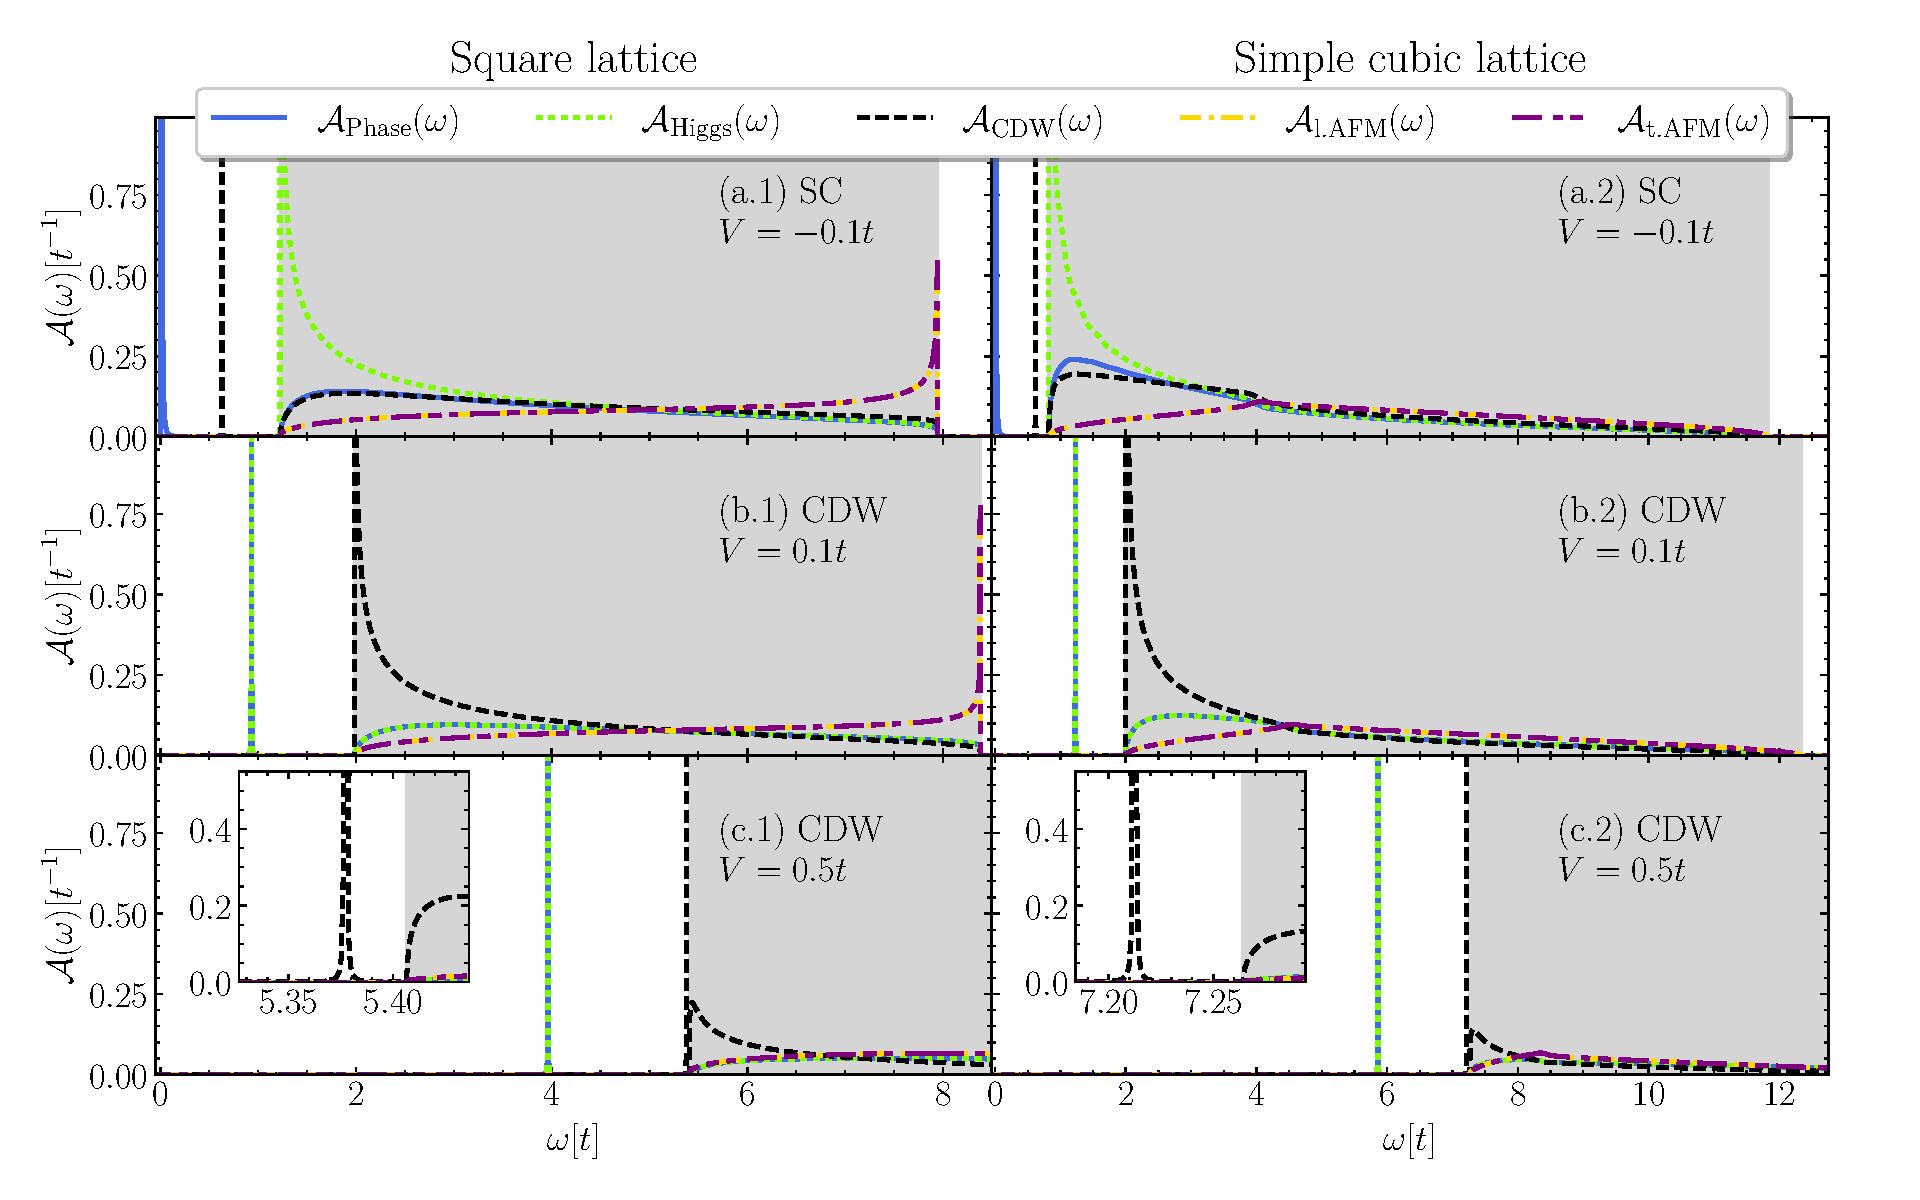
\includegraphics[width=.98\textwidth]{plots/resolvent_overview_SC_CDW.pdf}
    \caption{Spectral functions of the operators listed in Eq.~\eqref{eqn:resolvent_bases}.
    The left column shows the results for the square lattice and the right column for the simple cubic lattice.
    The left edge of each plot is at $-0.05t$  in order to improve the visibility of the phase peak at zero frequency
		($\hbar$ is set to unity). The gray area marks the two-particle continuum.
    The parameters are set to $U=-2.5t$ and $N_\gamma = 6000$, while $V$ is varied according to the legends.
    The panels show the spectral functions in the SC phase (a) and in the CDW phase, (b) and (c), respectively.}
    \label{fig:resolvent_overview_SC}
\end{figure*}

\begin{figure*}
    \centering
    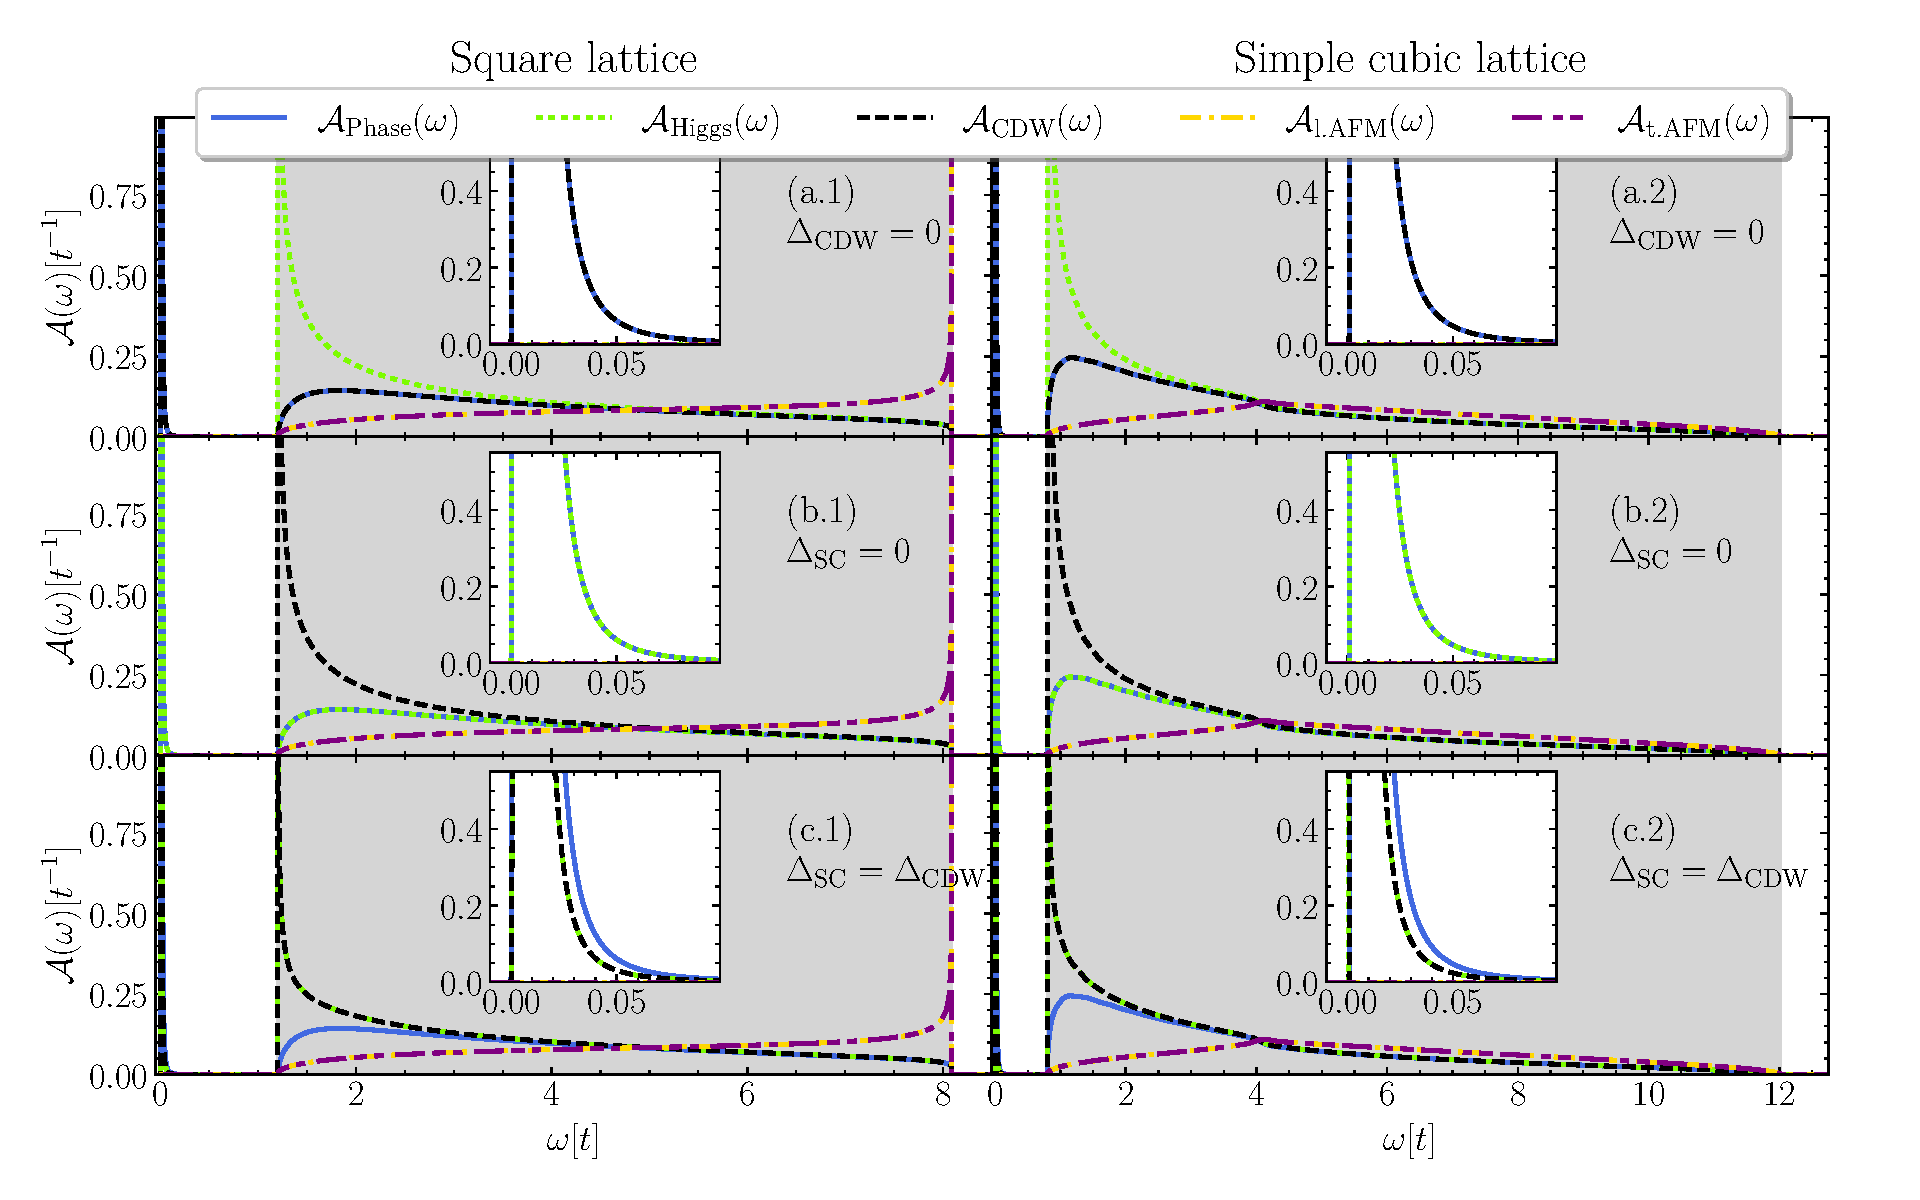
\includegraphics[width=.98\textwidth]{plots/resolvent_overview_V0.pdf}
    \caption{Same as Fig.\ \ref{fig:resolvent_overview_SC} except that  $V=0$, i.e., 
		SC and CDW order can coexist due to the SO(4) symmetry.
    Since the ratio of $\Delta_\text{SC}$ to $\Delta_\text{CDW}$ can be chosen arbitrarily, 
    we show in (a) the spectral functions for $\Delta_\text{CDW} = 0$ and in (b) for $\Delta_\text{SC} = 0$ while we distribute the gap equally in (c).}
    \label{fig:resolvent_overview_V0}
\end{figure*}

\begin{figure*}
    \centering
    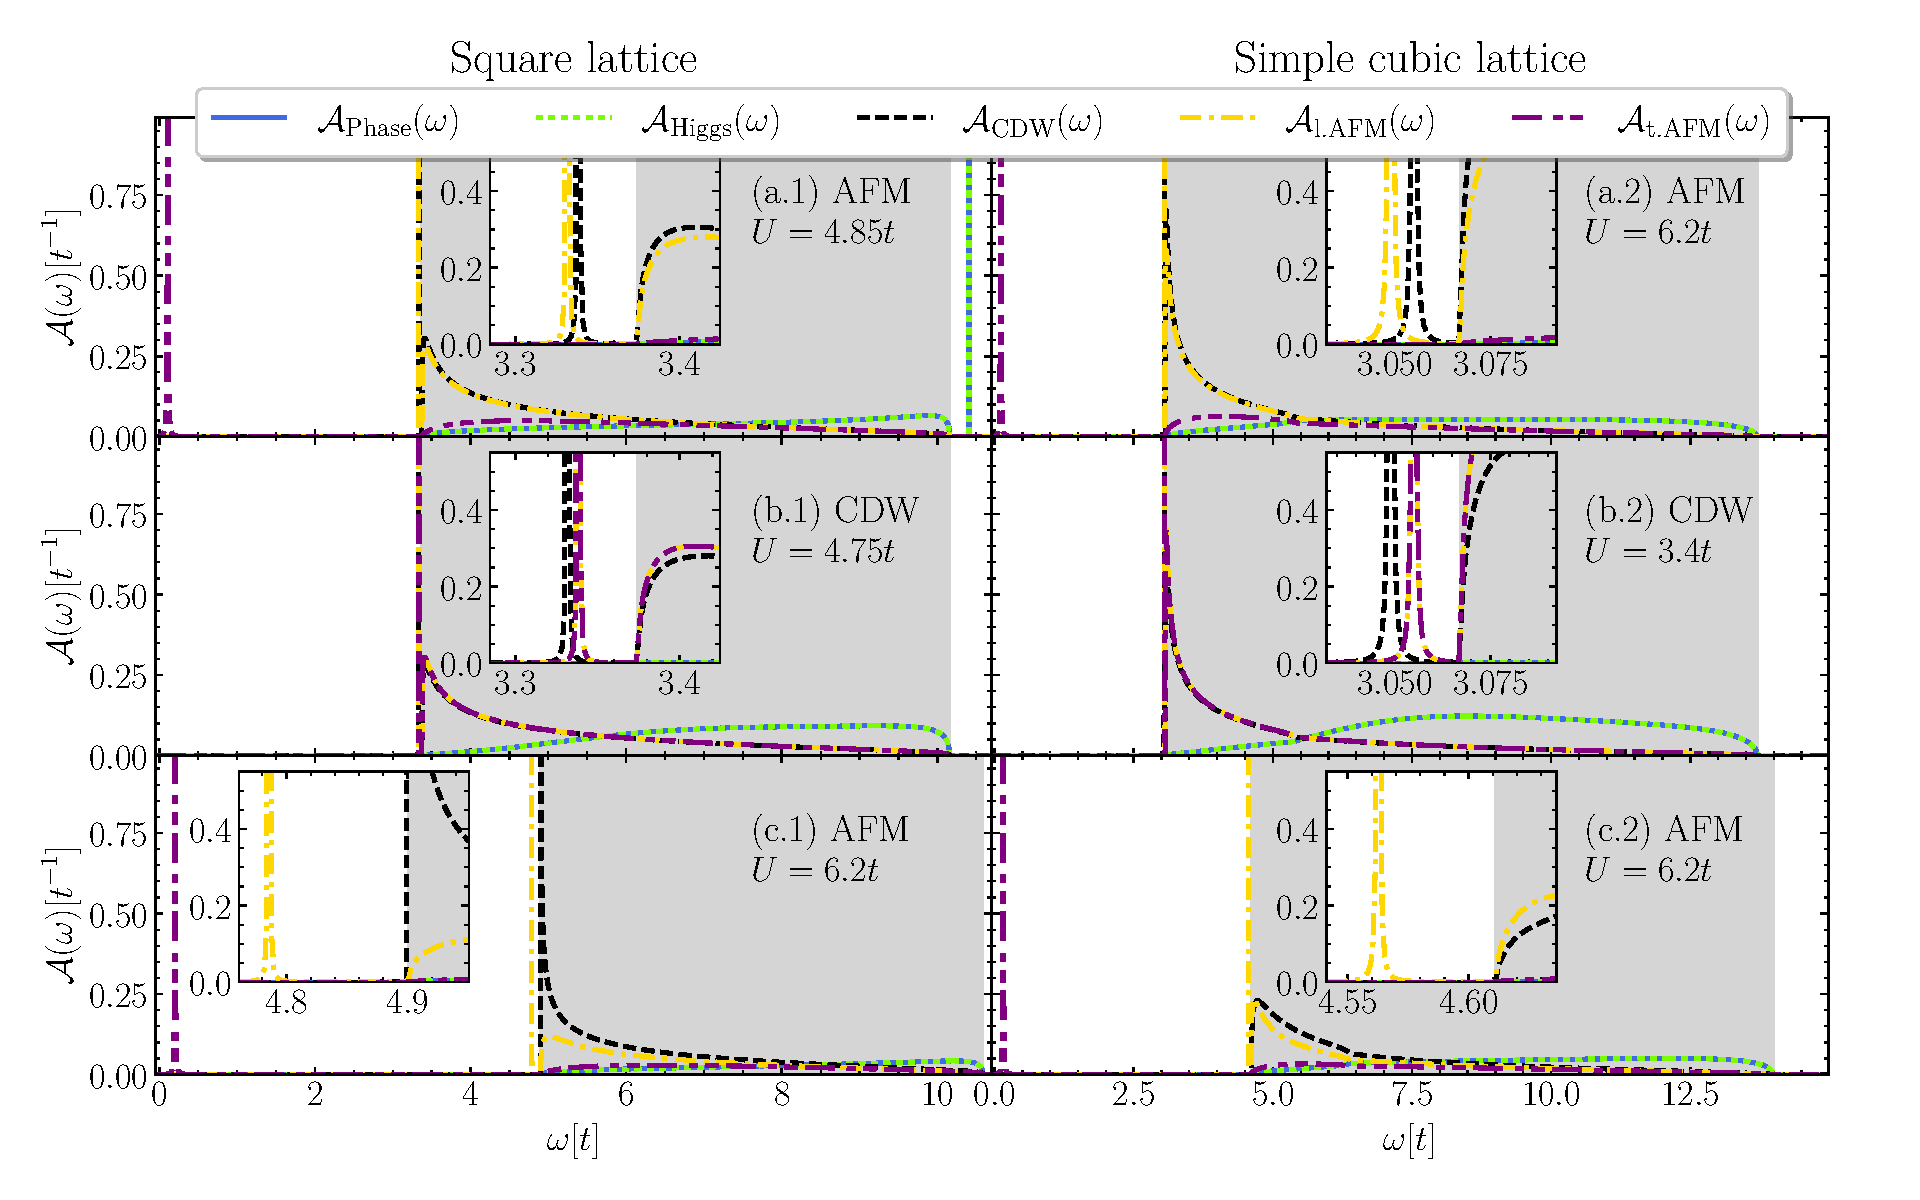
\includegraphics[width=.98\textwidth]{plots/resolvent_overview_AFM_CDW.pdf}
    \caption{\red{Die ersten beiden Reihen muessen getauscht werden. Stimmt dann der Text?} 
    \blue{Ich hab dir offenbar tatsächlich den falschen Plot geschickt... 
    Das ist der Plot der auf dem Poster ist, hier hatte ich eigentlich einen 4 Zeilen-Plot angedacht.}
		Same as Fig.\ \ref{fig:resolvent_overview_SC} except that we are focusing 
		on the AFM-CDW phase transition.
    For the square lattice, we set $V=1.2t$, and for the simple cubic lattice, $V=0.8t$. 
		This choice yields the phase transition at $U=4.8t$ for both lattices.
    The panels (a) and (c) show the spectral functions in the AFM phase and the 
		panels (b) and (d) in the CDW phase.}
    \label{fig:resolvent_overview_AFM}
\end{figure*}

\begin{figure*}
    \centering
    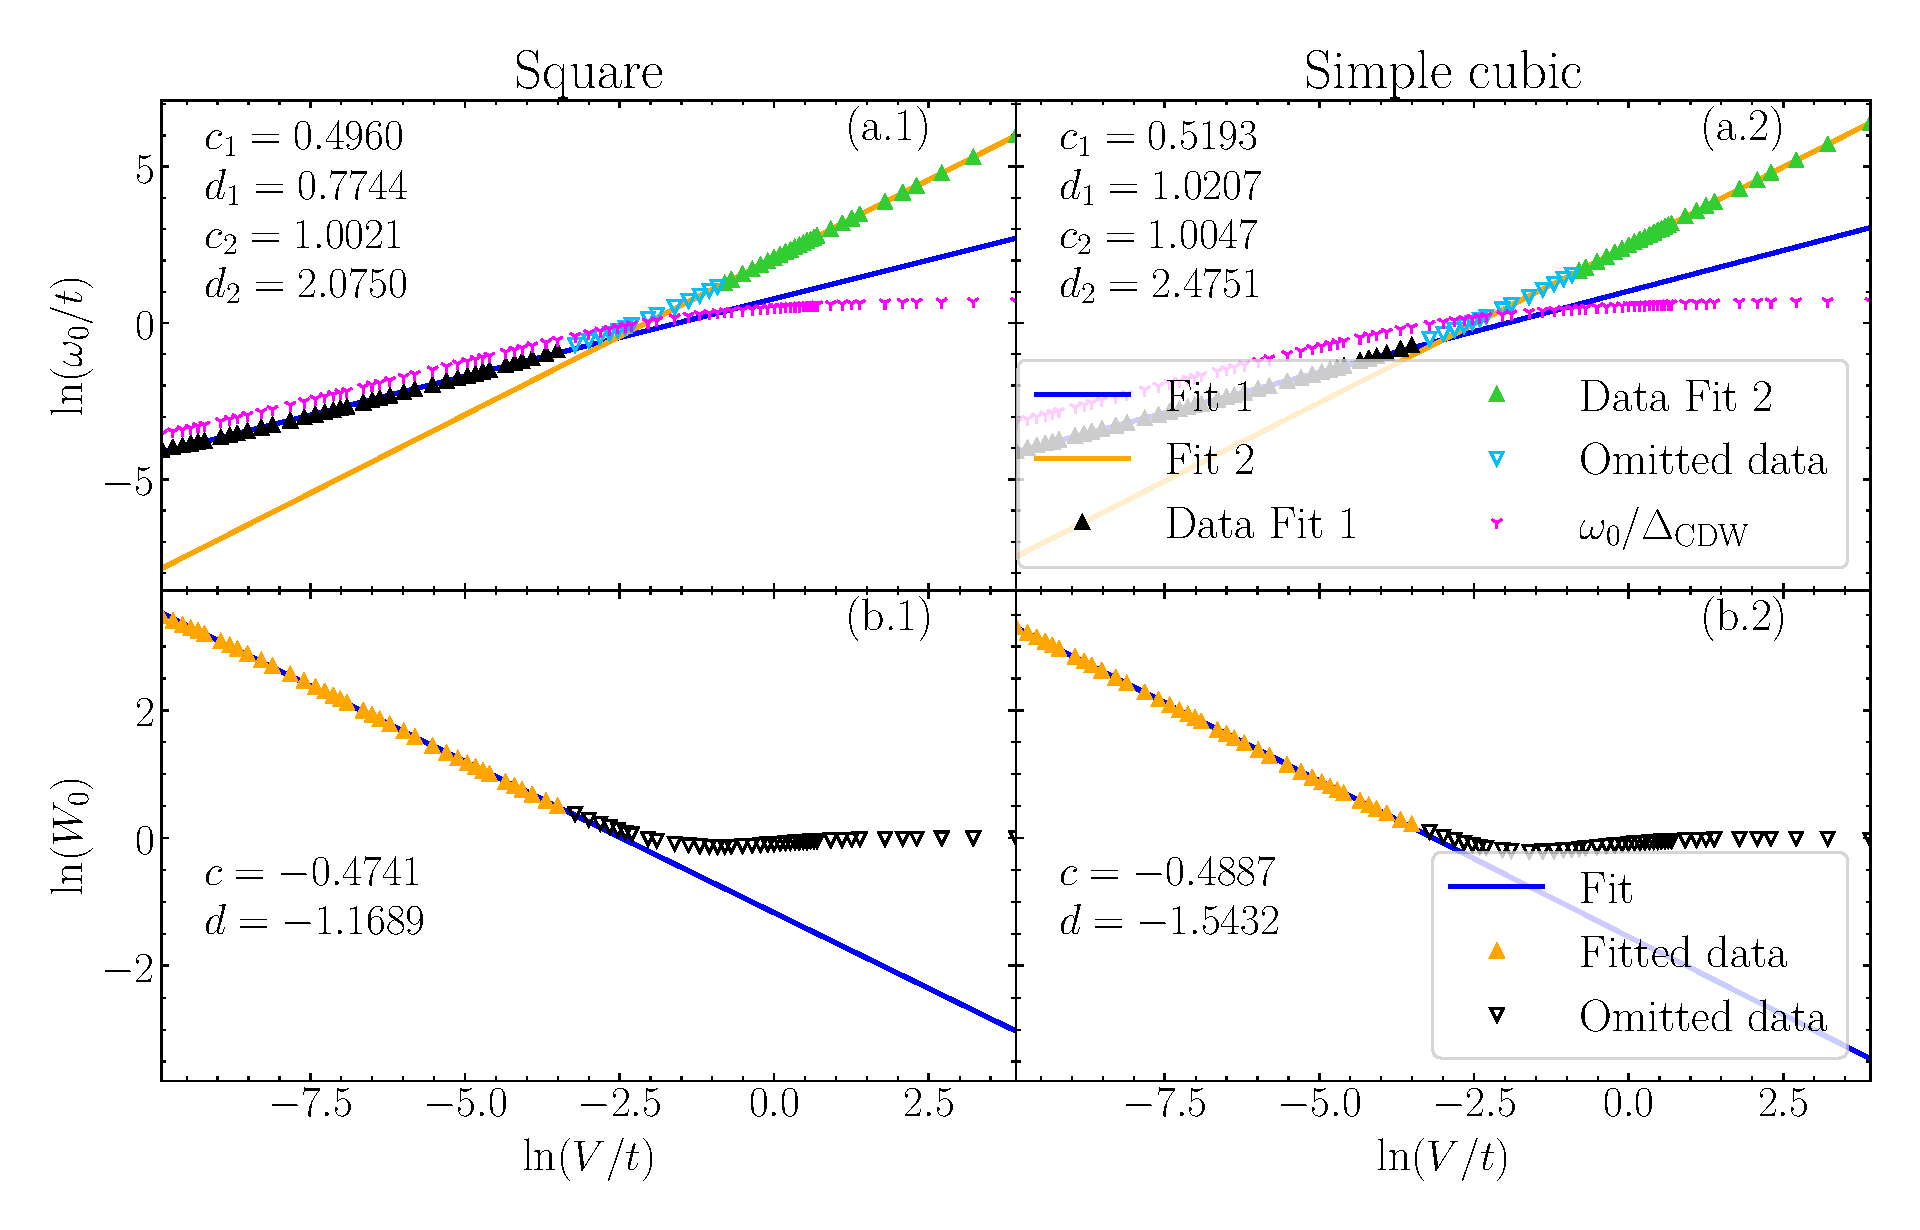
\includegraphics[width=.98\textwidth]{plots/sc_peak_in_cdw.pdf}
    \caption{The upper panels (a) show double logarithmic plots of the positions $\omega_0$ of the peak in $\spectral{SC}$ in the CDW phase 
    while the lower panels (b) show their respective weights $W_0$.
    In the upper panels, the pink markers additionally show the peak position divided by the gap $\omega_0 / \Delta_\text{CDW}$. 
    The left column shows the results for the square lattice and the right column for the simple cubic lattice at $U=-2.5t$. 
    The fits are linear in the double logarithmic plot, i.e., $y(V) = e^d V^c$, and the parameters are indicated in the panels.}
    \label{fig:sc_in_cdw_behavior}
\end{figure*}

\begin{figure*}
    \centering
    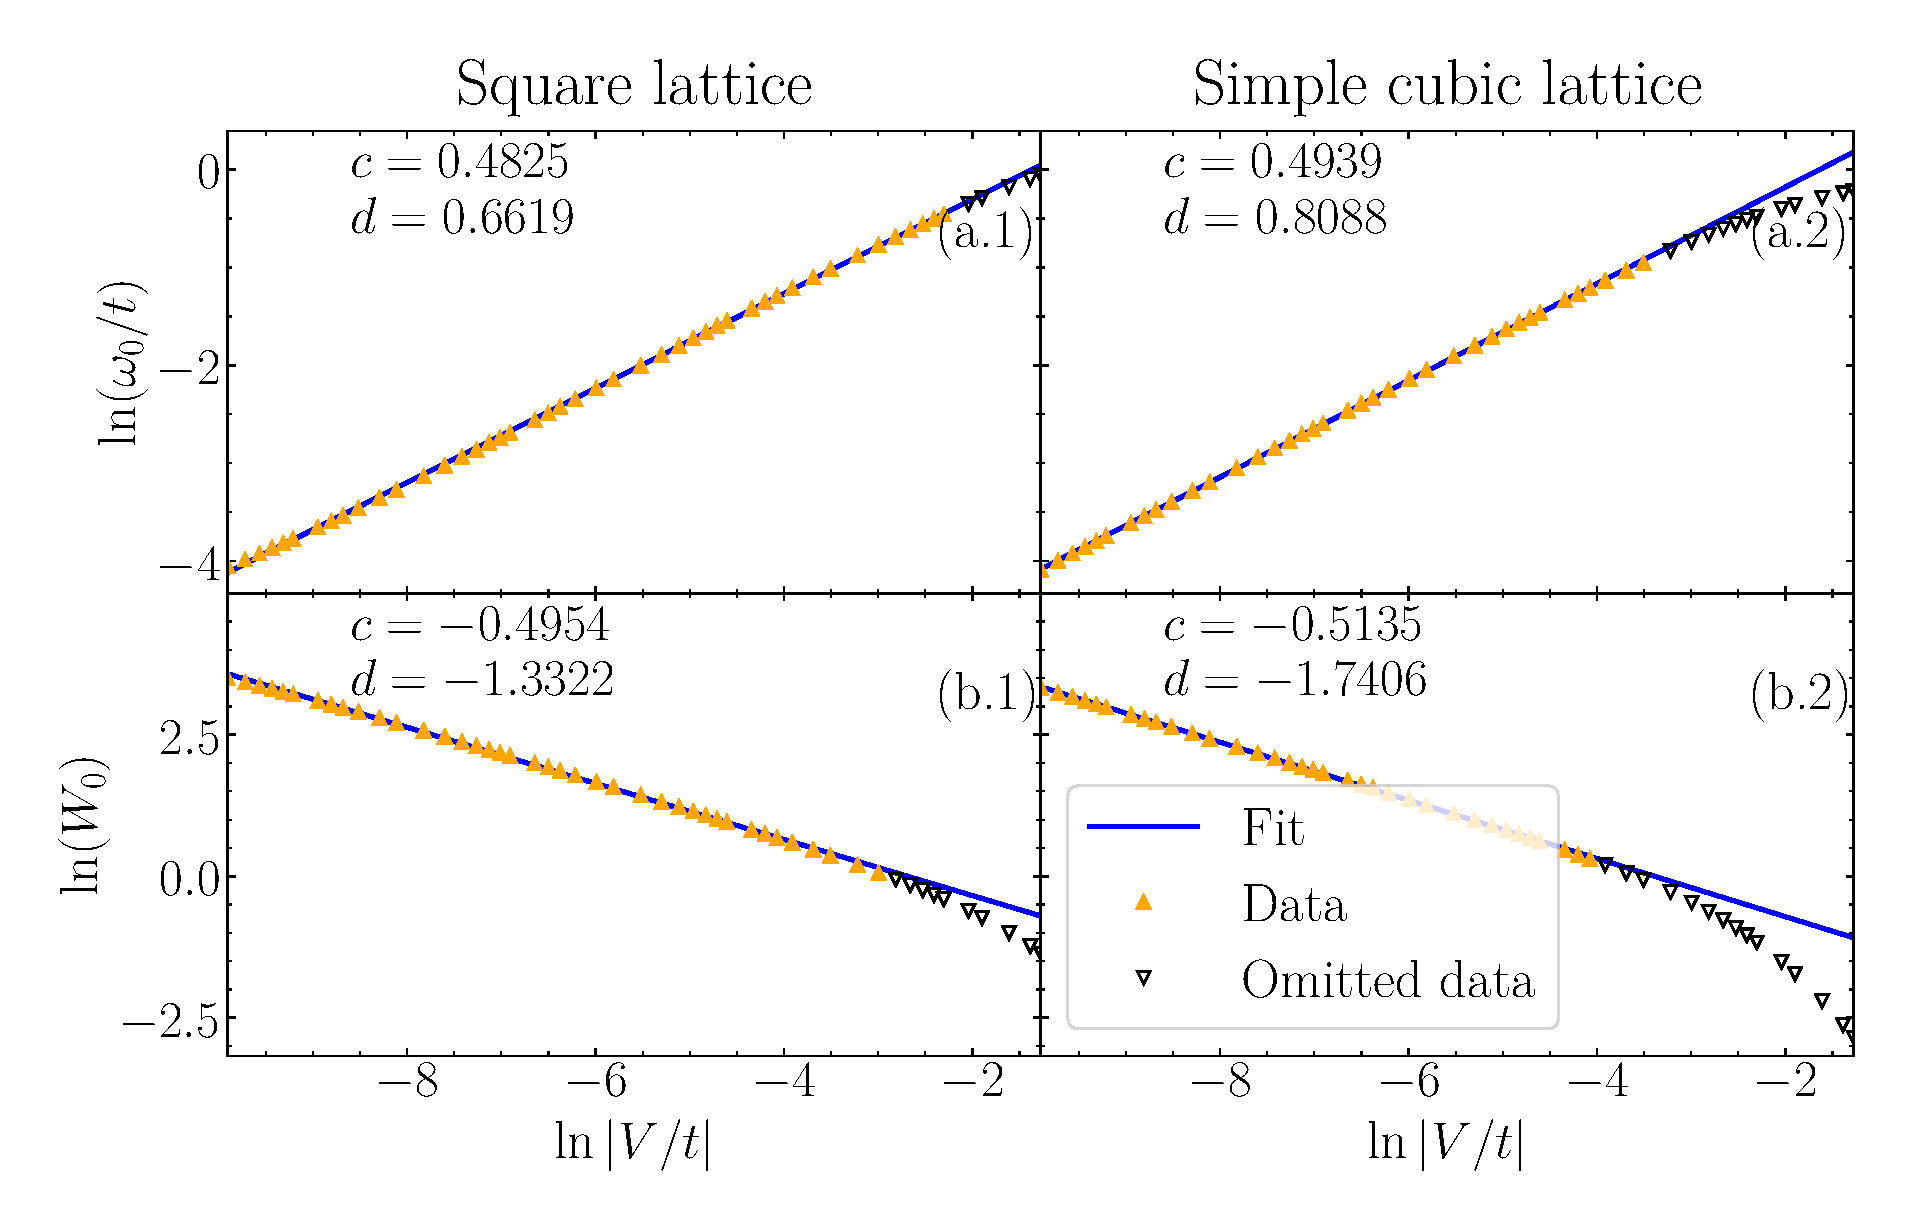
\includegraphics[width=.98\textwidth]{plots/cdw_peak_in_sc.pdf}
    \caption{Same as in Fig.\ \ref{fig:sc_in_cdw_behavior}, but for the peak in $\spectral{CDW}$ 
		in the SC phase, i.e., for $V<0$.}
    \label{fig:cdw_in_sc_behavior}
\end{figure*}

\begin{figure*}
    \centering
    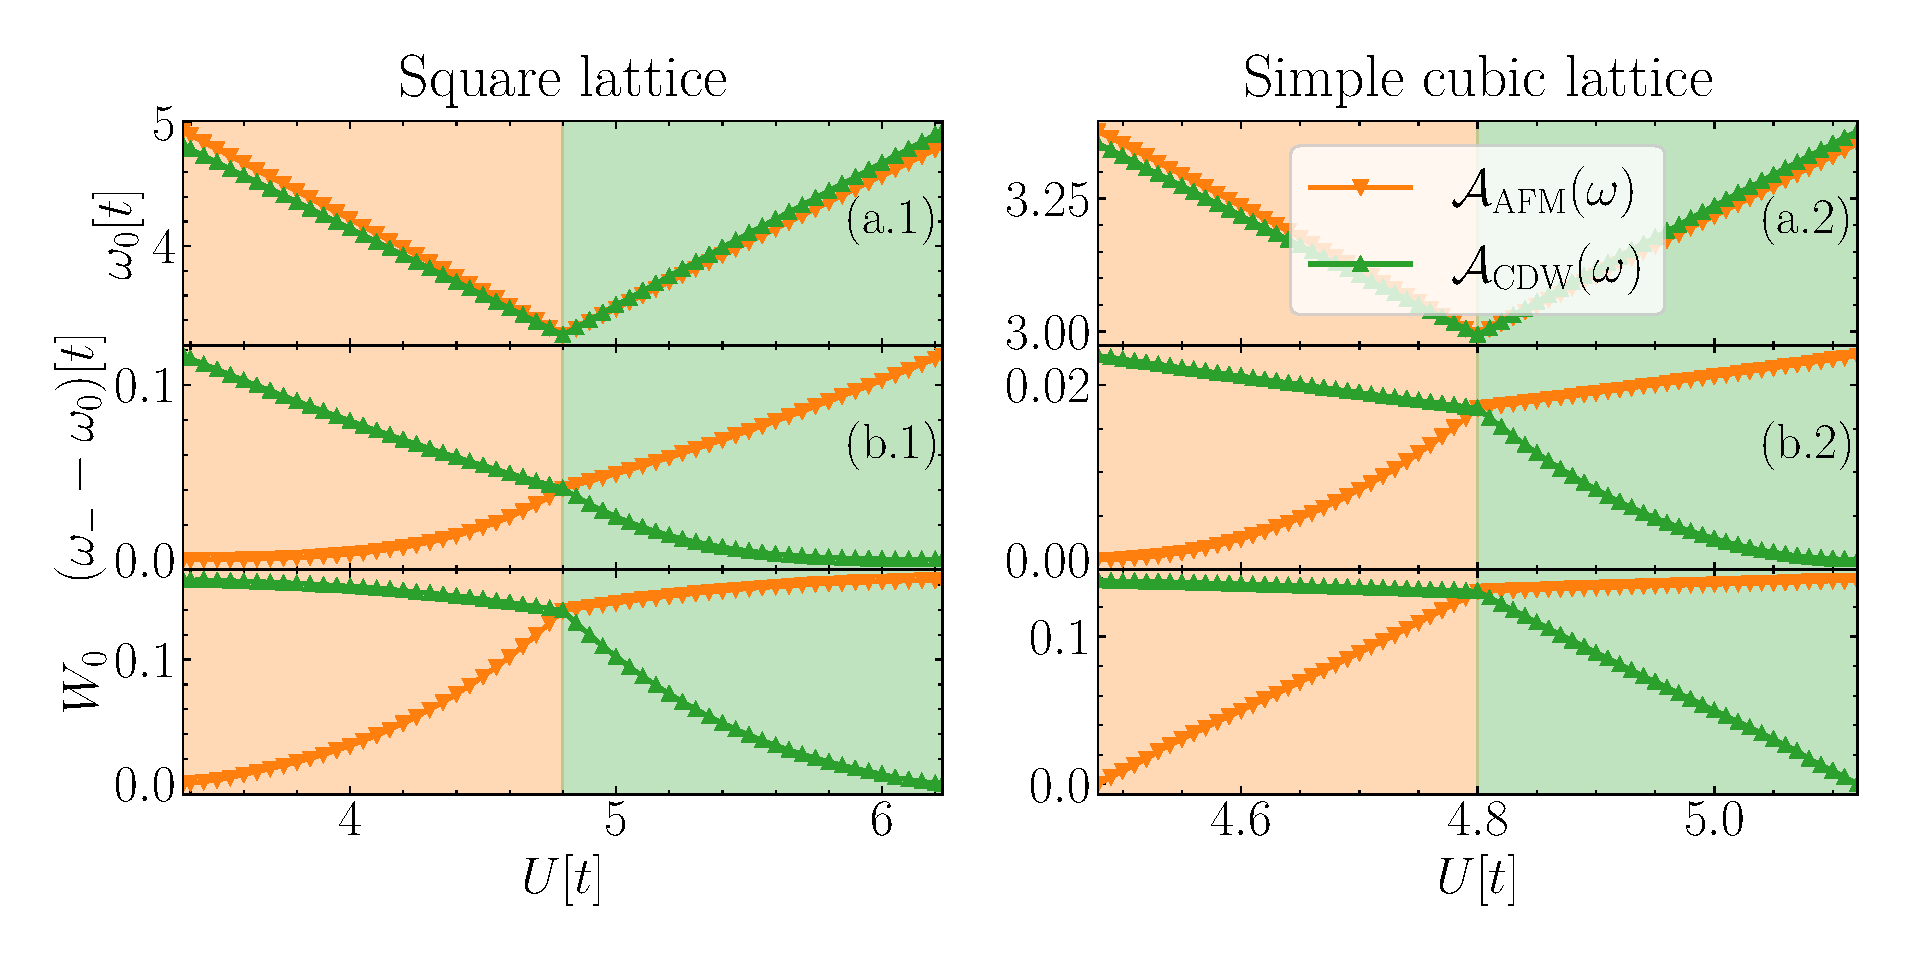
\includegraphics[width=.98\textwidth]{plots/afm_cdw_peaks_overview.pdf}
    \caption{The upper panels (a) show plots of the positions $\omega_0$ of the peak in $\spectral{CDW}$ (orange lines) 
		and $\spectral{l.AFM}$ (green lines) close to the corresponding phase transition 
		at $U = 4.8t$.   Again, we choose $V=1.2t$ for the square lattice (left column) and $V=0.8t$ for the simple cubic lattice (right column), respectively.
    The middle panels (b) depict the peak positions relative to the lower edge of the two-particle continuum 
		$\omega_-$, while the bottom panels (c) show the peak weights.
    The shadings indicate the phase in which the system is. Green represents AFM while orange represents CDW.
    Note the difference in the scales for the two lattices.}
    \label{fig:afm_cdw_peaks_overview}
\end{figure*}


\begin{figure*}
    \centering
    \includegraphics[width=.98\textwidth]{plots/afm_cdw_peaks_details.pdf}
    \caption{\red{Muss es im log-Argument nicht $U_0-U$ heissen, um klar zu sein?}  \blue{Wir plotten $U\in(U_0, 4.8t)$, also $U_0 < U$}
		The upper panels (a) show double logarithmic plots of the positions $\omega_0$ 
		of the peak in $\spectral{l.AFM}$ relative to the lower edge of the two-particle continuum $\omega_-$.
    The lower panels (b) depict the respective weights $W_0$.
    Again, we choose $V=1.2t$ for the square lattice (left column) and 
		$V=0.8t$ for the simple cubic lattice (right column), respectively.
    The interaction $U_0$ denotes the highest value of $U$ for which 
		there is no peak below the two-particle continuum, i.e., for $U> U_0$ a peak occurs.
		\red{Ja, was gilt? Wann gibt's einen Peak, wann nicht? Bitte konsistent im ganzen Artikel bezeichnen.}
    For the square lattice, we find $U_0 \approx 3.372t$ and for the simple cubic lattice $U_0 \approx 4.479t$.
    The parameter range depicted here places the system within the CDW phase.
    The fits are of the same kind as in Fig.\ \ref{fig:sc_in_cdw_behavior}.}
    \label{fig:afm_cdw_peaks_details}
\end{figure*}

%%%%%%%%%%%%%%%%%%%%%%%%%%%%%%%%%%%%%%%%%%%%%%%%%%%%%%%%%%%%%%%%%%%%%%%%%%%%%%%%%%%%%%%%%%%%%%%%%%%%%%%%%%%%%%%%%%%%%
%%%%%                                                  Figures                                                  %%%%%
%%%%%%%%%%%%%%%%%%%%%%%%%%%%%%%%%%%%%%%%%%%%%%%%%%%%%%%%%%%%%%%%%%%%%%%%%%%%%%%%%%%%%%%%%%%%%%%%%%%%%%%%%%%%%%%%%%%%%

%%%%%%%%%%%%%%%%%%%%%%%%%%%%%%%%%%%%%%%%%%%%%%%%%%%%%%%%%%%%%%%%%%%%%%%%%%%%%%%%%%%%%%%%%%%%%%%%%%%%%%%%%%%%%%%%%%%%%
%%%%%%%%%%%%%%%%%%%%%%%%%%%%%%%%%%%%%%%%%%%%%%%%%%%%%%%%%%%%%%%%%%%%%%%%%%%%%%%%%%%%%%%%%%%%%%%%%%%%%%%%%%%%%%%%%%%%%
%%%%%                                                  Results                                                  %%%%%
%%%%%%%%%%%%%%%%%%%%%%%%%%%%%%%%%%%%%%%%%%%%%%%%%%%%%%%%%%%%%%%%%%%%%%%%%%%%%%%%%%%%%%%%%%%%%%%%%%%%%%%%%%%%%%%%%%%%%
%%%%%%%%%%%%%%%%%%%%%%%%%%%%%%%%%%%%%%%%%%%%%%%%%%%%%%%%%%%%%%%%%%%%%%%%%%%%%%%%%%%%%%%%%%%%%%%%%%%%%%%%%%%%%%%%%%%%%

\section{Results}
\label{sec:results}


We investigate four different diagonal Green's functions $G_{AA^\dagger}(\omega + \im 0^+)$ with
\begin{subequations}
    \label{eqn:resolvent_bases}
    \begin{align}
        A_\text{Higgs} &= \frac{1}{\sqrt{N}} \sum_{\vk} \left( f_{\vk} + f_{\vk}^\dagger \right)  
            = \int_{-1}^1 \dgamma \left( f_{\gamma} + f_{\gamma}^\dagger \right) ,\\
        A_\text{Phase} &= \frac{i}{\sqrt{N}} \sum_{\vk} \left( f_{\vk} - f_{\vk}^\dagger \right) = 
				\int_{-1}^1 \dgamma \left( f_{\gamma} - f_{\gamma}^\dagger \right) ,\\
        A_\text{CDW}   &= \frac{1}{\sqrt{N}} \sum_{\vk} \left( g_{\vk \up} + g_{\vk \down} \right) = 
				\int_{-1}^1 \dgamma \left( g_{\gamma \up} + g_{\gamma \down} \right) ,\\
        A_\text{l.AFM}   &= \frac{1}{\sqrt{N}} \sum_{\vk} \left( g_{\vk \up} - g_{\vk \down} \right) = 
				\int_{-1}^1 \dgamma \left( g_{\gamma \up} - g_{\gamma \down} \right) , \\
        A_\text{t.AFM}   &= \frac{1}{\sqrt{N}} \sum_{\vk} \left( \tau_{\vk} + \tau_{\vk}^\dagger \right) = 
				\int_{-1}^1 \dgamma \left( \tau_{\gamma \up} + \tau_{\gamma \down} \right) ,
    \end{align}
\end{subequations}
where $N$ is the number of lattice sites in the system. 
Each of these operators generates a different kind of collective mode.
The first operator excites the amplitude mode of the $s$-wave superconducting state
while the second one excites the phase mode \cite{Fan22}.
The remaining two operators induce the collective behavior of the CDW and AFM order, respectively.
This means these Green's functions are the susceptibilities towards alternating local potential (CDW) or
alternating magnetic field (AFM).
Below, we refer to the Green's functions of these operators by
$\mathcal{G}_{\alpha}(\omega) = G_{A_\alpha A_\alpha^\dagger}(\omega)$ 
with $\alpha \in \{ \text{Higgs}, \text{Phase}, \text{CDW}, \text{l.AFM}, \text{t.AFM} \}$.
Furthermore, we use $\text{SC}$ when the Higgs and phase mode yield the same spectral function and
$\text{AFM}$ when longitudinal and transversal magnons yield the same spectral function.

The operators in \eqref{eqn:resolvent_bases} are Hermitian and of bosonic character. 
This means that all spectral functions are antisymmetric \cite{rickayzen80}.
For this reason, we only show the part  $\omega \geq 0$ in our plots. 
Additionally, we add a small positive imaginary part of $10^{-5}t$ to $\omega$ 
in order to plot the $\delta$ peaks as Lorentzians.
We analyze the effect of different numbers of sampling points $N_\gamma$ in App.\ \ref{sec:finite_size}.

%%%%%%%%%%%%%%%%%%%%%%%%%%%%%%%%%%%%%%%%%%%%%%%%%%%%%%%%%%%%%%%%%%%%%%%%%%%%%%%%%%%%%%%%%%%%%%%%%%%%%%%%%%%%%%%%%%%%%
%%%%%                                              Classification                                               %%%%%
%%%%%%%%%%%%%%%%%%%%%%%%%%%%%%%%%%%%%%%%%%%%%%%%%%%%%%%%%%%%%%%%%%%%%%%%%%%%%%%%%%%%%%%%%%%%%%%%%%%%%%%%%%%%%%%%%%%%%

\subsection{Classification of the spectral functions}

Let us describe the spectral functions 
$\mathcal{A}_\alpha (\omega) = - (1/\pi) \Im [\mathcal{G}_\alpha (\omega + \im 0^+)]$ of
the operators above in the various phases.
Fig.\ \ref{fig:resolvent_overview_SC} shows them at $U = -2.5t$ in the SC ($V=-0.1t$) and  in the 
CDW ($V=0.1t$ and $V=0.5t$) phase.

There are a variety of different features. 
The results for the lattices in 2D and 3D are very similar and differ only quantitatively.
In the SC phase, see Fig.\ \ref{fig:resolvent_overview_SC}(a), 
there is a sharp peak located at $\omega=0$ in $\spectral{Phase}$ and a 
singularity in $\spectral{Higgs}$ located at $\omega=2\Delta_\text{SC}$.
We identify them with the well-known Anderson-Bogoliubov mode and Higgs mode, respectively, in superconductors 
\cite{Bogoljubov1958,Anderson58,Brieskorn74,Schmid1975,simanek1975,schon76,Kulik1981,Maiti2015,Sun2020,Fan22,Schmid1975,Varma02,Cea14,Measson14,Tsuji15,Krull16,Mueller2019,Schwarz20}.
The former must not have any weight because of the antisymmetry of the spectral function.
The peak itself is located at zero energy because the model \eqref{eqn:full_hamiltonian} 
describes a neutral superfluid without coupling of the phase of the order parameter to the electromagnetic fields.
Therefore, this phase may be chosen arbitrarily, and changing it requires no energy 
which ultimately induces a Goldstone mode to exist \cite{Goldstone1961,Anderson63}.

To characterize the occurring peaks that lie outside the two-particle continuum, we inspect the real part of the Green's function.
We plot it in the vicinity of the peaks with a double logarithmic scale and fit 
the result linearly $y = ax + b$ to obtain its power-law behavior.
The real part is related to the imaginary part via the Kramers-Kronig relations.
Specifically, if the imaginary part is a $\delta$ distribution, the real part will be proportional to $1/\omega$, i.e., $a=-1$, and the peak has the weight $W_0 = \exp(b)$.
Furthermore, an exponent of $a=-2$ corresponds to the 
derivative of the $\delta$ distribution, i.e., $\delta'(\omega)$.
The fits themselves are given in App.\ \ref{sec:fit_greens_functions}.

This analysis yields that the real part of $\greens{Phase}$ near $\omega=0$ behaves like
$1/\omega^2$ showing that the peak in $\spectral{Phase}$ is the derivative of a $\delta$ distribution.
The weight of such a peak is given by the integral $\int \delta'(\omega) \mathrm{d}\omega = 0$ and thus
vanishes in accordance with expectations.

The singularity in $\spectral{Higgs}$ behaves like $1/\sqrt{\omega - 2 \Delta_\text{SC}}$.
Previous studies on the dynamics of the order parameter found dephasing oscillations after a quench.
These oscillations have the frequency $\Omega = 2 \Delta_\text{SC}$ and fall off like
$1/\sqrt{t}$ \cite{Volkov73,Kulik1981,Yuzbashyan06}.
An inverse Fourier transform of $\spectral{Higgs}$ yields precisely this behavior, 
thereby corroborating our results.

In the CDW phase, see panels (b) and (c) of Fig.\ \ref{fig:resolvent_overview_SC},
both spectral functions $\spectral{Higgs}$ and $\spectral{Phase}$ become identical and display a $\delta$ peak below the two-particle continuum.
In this case, both modes describe a cooperon, i.e., a bound state of two electrons or two holes.
Following the Landau theory for continuous phase transitions, it is to be expected 
that both excitations show the same spectral behavior. 
If the free energy is expanded in powers of the order parameter 
\begin{equation}
    f(\Delta_\text{SC}) \approx r |\Delta_\text{SC}|^2 + \frac{u}{2} |\Delta_\text{SC}|^4,
\end{equation}
with  $u > 0$. For $r<0$, the system is in the SC phase and $\Delta_\text{SC}$ is finite.
Then it makes a difference if one excites \emph{along} $\Delta_\text{SC}$ in the complex plane (Higgs mode)
or \emph{perpendicular} to it (phase mode). For $r>0$, however, the order vanishes, $\Delta_\text{SC}=0$,
and no distinction between Higgs and phase mode can be made \cite{Coleman2015}. 
Both possible excitation processes have to overcome the same energy. 

In the SC phase, $\spectral{CDW}$ features a $\delta$ peak below the continuum corresponding to the finite energy necessary to excite the electronic density modulation of CDW type.
This mode corresponds to the creation of an exciton since it results from a bilinear operator with
creation and annihilation fermionic operator so that it represents a bound electron-hole pair.
For moderate values of $V>0$, i.e., in the CDW phase, see panel (b) at $V=0.1t$, the CDW spectral function 
shows a singularity at $\omega=2\Delta_\text{CDW}$.
This mode moves out of the two-particle continuum upon increasing $V$ 
and becomes a proper $\delta$ peak, see panel (c) of Fig.\ \ref{fig:resolvent_overview_SC} at $V=0.5t$.

The spectral functions $\spectral{t.AFM}$ and $\spectral{l.AFM}$ are identical and restricted to 
the continuum for both phases and both lattices.
This can be understood by the same argument used for the identity of 
$\spectral{Phase}$ and $\spectral{Higgs}$ outside of the SC phase:
If no AFM order is present, there is no distinction between a longitudinal and a transversal excitation. 
The same amount of energy is required to create any such excitation which is a magnon
or paramagnon if there is no long-range AFM order.
For the square lattice, there is a singularity located at the upper edge of the two-particle continuum.
But this does not occur in the 3D case. Including lifetime effects, sharp features at the upper
edge of the continuum are expected to be smeared out anyway.

%%%%%%%%%%%%%%%%%%%%%%%%%%%%%%%%%%%%%%%%%%%%%%%%%%%%%%%%%%%%%%%%%%%%%%%%%%%%%%%%%%%%%%%%%%%%%%%%%%%%%%%%%%%%%%%%%%%%%

At $V=0$, the SC and the CDW order can coexist due to the SO(4) symmetry. 
In this phase, the mean-field single-particle energies are given by
\begin{equation}
    E_{\pm} = \pm \sqrt{\epsilon^2 + |\Delta_\text{CDW}|^2 + |\Delta_\text{SC}|^2}.
\end{equation}
This means that the proper order parameter is $\Delta_\text{tot} 
\coloneqq \sqrt{|\Delta_\text{CDW}|^2 + |\Delta_\text{SC}|^2}$.
Here, $\Delta_\text{CDW}$ and $\Delta_\text{SC}$ can change arbitrarily without affecting the system's energy as long as $\Delta_\text{tot}$ remains constant.
This degeneracy of both phases is rigorously exact due to the SO(4) symmetry \cite{yang90}. 

In Fig.\ \ref{fig:resolvent_overview_V0}, we show the spectral functions for $U=-2.5t$ and $V=0$.
The different panels correspond to different choices for $\Delta_\text{CDW}$ and $\Delta_\text{SC}$.
First, in panel (a), we set $\Delta_\text{CDW} = 0$.
This results in a purely superconducting phase with the same features as in 
Fig.\ \ref{fig:resolvent_overview_SC}(a).
The peak in $\spectral{CDW}$ moves to $\omega=0$ because it does not cost energy to enhance the CDW order parameter
if it is compensated by a reduction of the SC order parameter. 
In fact, $\spectral{CDW}$ and $\spectral{Phase}$ are identical since they are linked by the SO(4) symmetry.

Second, panel (b) shows the spectral functions for $\Delta_\text{SC} = 0$, i.e., in a purely charge-ordered phase.
Similar to before, there is not much change compared to Fig.\ \ref{fig:resolvent_overview_SC}(b).
The spectral functions $\spectral{Higgs}$ and $\spectral{Phase}$ are still identical since no
SC order is present. Both exhibit a sharp peak at $\omega=0$ proportional to $\delta'(\omega)$
which reflects that an SC order can be introduced without energy cost if compensated by a reduction of the CDW order.

Last, we choose $\Delta_\text{CDW} = \Delta_\text{SC}$ in panel (c).
For this specific ratio of $\Delta_\text{CDW}$ and $\Delta_\text{SC}$, 
$\spectral{Higgs}$ and $\spectral{CDW}$ are identical.
Choosing a different ratio yields qualitatively the same results, but the peaks differ in magnitude.
Both spectral functions have a peak at $\omega = 0$ proportional to $\delta'(\omega)$
and a singularity at the lower edge of the two-particle continuum $\omega = 2\Delta_\text{tot}$.
These singularities behave like $1/\sqrt{\omega - 2 \Delta_\text{tot}}$.
Varying the ratio of the two gap parameters allows one to
switch between $\spectral{Higgs}$ and $\spectral{CDW}$ continuously.

We attribute the peak in the amplitude spectral functions at $\omega=0$ 
to the freedom to vary the order parameters, i.e., 
diminishing one and increasing the other while keeping $\Delta_\text{tot}$ 
constant so that the system stays in its ground states. 
In the pure SC phase, we find this peak only in $\spectral{CDW}$.
This can be understood as follows: The operator $A_\text{CDW}$ in \eqref{eqn:resolvent_bases} 
creates an exciton and thereby increases $|\Delta_\text{CDW}|$.
This can be achieved without increasing the energy by lowering $\Delta_\text{SC}$.
However, the reversed argument is not true: Since $\Delta_\text{CDW}$ is already 0, 
creating another Cooper pair by virtue of $A_\text{Higgs}$ always increases $\Delta_\text{tot}$ and thus 
requires a minimum energy of $2 \Delta_\text{tot}$.
The analogous argument holds for the pure CDW phase.
If, however, both orders are present, the system can shift between them arbitrarily 
by creating either kind of excitation.
Hence, in this case, we find a peak at $\omega=0$ in both spectral functions.

The spectral function $\spectral{Phase}$ behaves as it does in the pure SC phase. 
It has only a peak at $\omega = 0$ that is associated with the freedom of choice
of the phase of $\Delta_\text{SC}$.

%%%%%%%%%%%%%%%%%%%%%%%%%%%%%%%%%%%%%%%%%%%%%%%%%%%%%%%%%%%%%%%%%%%%%%%%%%%%%%%%%%%%%%%%%%%%%%%%%%%%%%%%%%%%%%%%%%%%%

Finally, we investigate the same spectral functions close to the AFM-CDW phase transition
as depicted in Fig.\ \ref{fig:resolvent_overview_AFM}.
We choose $V=1.2t$ for the square lattice and $V=0.8t$ for the simple cubic lattice so that
the phase transition is located at $U=4.8t$ in both cases. 
The panels (a) and (b) show the system close to the phase transition at $U=4.8t \pm 0.05t$.
Again, the SC-related spectral functions are identical in the CDW and the AFM phases
due to the absence of a finite SC order.
Within the continuum, their weight is shifted towards the upper edge.
On the square lattice only, there is a peak above the continuum.
It is likely to be smeared out if lifetime effects were included.
In the AFM phase, both $\spectral{l.AFM}$ and $\spectral{CDW}$ have a peak close to, but yet below, the two-particle continuum. 
The peak of the former is at a lower energy than the peak of the latter.
In the CDW phase, this behavior is reversed, i.e., the peak of $\spectral{CDW}$ lies lower
than the one in $\spectral{l.AFM}$.
Analyzing the power-law behavior of the real part described above, see also
App.\ \ref{sec:fit_greens_functions}, we confirm that these peaks are $\delta$ peaks.
Moving further away from the phase transition, here $U=6.2t$ in panels (c) \blue{and $U=3.4t$ in panels (d)}
\red{Im Text war (d) benannt, aber das existiert ja nicht.}, 
the upper peak merges with the two-particle continuum while the lower one persists.
We emphasize that the spectral function of the transverse magnon $\spectral{t.AFM}$ always 
displays a $\delta'$ peak at $\omega=0$, independent of how far away the parameters are chosen
from the phase transition. This is the expected behavior of a Goldstone boson.


%%%%%%%%%%%%%%%%%%%%%%%%%%%%%%%%%%%%%%%%%%%%%%%%%%%%%%%%%%%%%%%%%%%%%%%%%%%%%%%%%%%%%%%%%%%%%%%%%%%%%%%%%%%%%%%%%%%%%
%%%%%                                                  SC-CDW                                                   %%%%%
%%%%%%%%%%%%%%%%%%%%%%%%%%%%%%%%%%%%%%%%%%%%%%%%%%%%%%%%%%%%%%%%%%%%%%%%%%%%%%%%%%%%%%%%%%%%%%%%%%%%%%%%%%%%%%%%%%%%%

\subsection{SC-CDW transition}

Having discussed the dominant peaks, we address their behavior when 
the system approaches the phase transition \blue{between the SC and CDW phase} at $V=0$ for $U=-2.5t$.
First, we investigate the identical peak in $\spectral{Phase}$ and $\spectral{Higgs}$, respectively, in the CDW phase.
The evolution of its position $\omega_0$ and its weight $W_0$ as a function of $V$ is depicted
double logarithmically in Fig.\ \ref{fig:sc_in_cdw_behavior}.
For $V \ll t$, the position increases with the square root of $V$. 
This behavior crosses over to a purely linear growth for large $V$.
The gap position $\omega_0$ relative to the gap $\Delta_\text{CDW}$ shows a plateau for large $V$ 
while leaving the square root behavior for small values of $V$ hardly altered.
The peak's weight $W_0$ decreases like $1/\sqrt{V}$ for $V \ll t$,
reaching a shallow minimum for intermediate valus of $V$, and 
eventually saturating at a constant value.

Summarizing, we see that for $V \ll t$ the peak position follows 
$\omega_0 = \alpha \sqrt{V}$ and its weight  $W_0 = \beta / \sqrt{V}$, 
where $\alpha$ and $\beta$ are some constants. Thus, we conclude $W_0 = \beta / (\alpha \omega_0)$. 
Furthermore, we know that the spectral functions are antisymmetric, i.e., we find
\bs
\begin{align}
    \mathcal{A}_\text{Phase} (\omega \ll t) &= W_0 (\delta (\omega - \omega_0) - \delta (\omega + \omega_0)) 
		\\
    &= - \frac{2\beta}{\alpha} \frac{\delta (\omega + \omega_0) - \delta (\omega - \omega_0)}{2\omega_0}.
\end{align} 
\es
Taking the limit $V \to 0$ corresponds to the limit $\omega_0 \to 0$, i.e., leading to a ratio tending to the
derivative
\begin{equation}
    \lim_{h \to 0} \frac{f(x + h) - f(x - h)}{2h} = f'(x).
\end{equation}
Applying this to the spectral peak yields
\begin{align}
    \lim_{\omega_0 \to 0} \mathcal{A}_\text{Phase} (\omega \ll t) = - \frac{2 \beta}{\alpha} \delta'(\omega),
\end{align}
confirming our previous analysis of the phase peak being proportional to  $\delta' (\omega)$.

%%%%%%%%%%%%%%%%%%%%%%%%%%%%%%%%%%%%%%%%%%%%%%%%%%%%%%%%%%%%%%%%%%%%%%%%%%%%%%%%%%%%%%%%%%%%%%%%%%%%%%%%%%%%%%%%%%%%%

Next, we analyze the peak in $\spectral{CDW}$ occurring if the system is in the SC phase for $V<0$.
A plot of its position $\omega_0$ and weight $W_0$ is given in Fig.\ \ref{fig:cdw_in_sc_behavior}.
The upper panels (a) and (b) depict the peak position and weight, respectively.
For $|V| \ll t$, the behavior of both of them is the same as for the 
previously discussed peak in $\spectral{SC}$ in the CDW phase.
Increasing $|V|$, the increase of the peak position slows down while the weights start to drop rapidly.
We cannot compute the Green's functions for even larger $|V|$ with $V<0$ because the dynamical matrix $\mM$ 
acquires negative eigenvalues below $V\approx -0.28t$ (square lattice) or $V\approx -0.34t$ (simple cubic lattice). 
We recall that this indicates that the assumed phase, i.e., the SC phase is not stable. 
Therefore, we conclude that for sufficiently negative values of $V$, 
the superconducting phase is not the true ground state as indicated by the red shading in Fig.\ \ref{fig:phase_diagram}.
Specifically, the region of the SC phase on the square lattice 
appears to be even smaller than shown by the $d_{x^2 -y^2}$ data from Ref.\ \cite{Micnas88b}.
Recently, there has been evidence for phase separation for negative values of $V$ 
on the square lattice, at least at finite temperature \cite{Linner23}. 
Thus, we interpret the negative eigenvalues in the dynamical matrix as indicators of phase separation. 
Physically, a strong attractive interaction clearly favors phase separation since the particles prefer to stay close together 
so it is highly plausible that they gather in one region of the sample while leaving the remainder essentially empty.
\red{Was ist in 3D - gibt es da nicht auch negative Eigenwerte usw.? Das solten wir dann hier
ebenfalls besprechen. Wo wollten wir denn die Diskussion des Tricks von Biermann publizieren?}


%%%%%%%%%%%%%%%%%%%%%%%%%%%%%%%%%%%%%%%%%%%%%%%%%%%%%%%%%%%%%%%%%%%%%%%%%%%%%%%%%%%%%%%%%%%%%%%%%%%%%%%%%%%%%%%%%%%%%
%%%%%                                                  AFM-CDW                                                  %%%%%
%%%%%%%%%%%%%%%%%%%%%%%%%%%%%%%%%%%%%%%%%%%%%%%%%%%%%%%%%%%%%%%%%%%%%%%%%%%%%%%%%%%%%%%%%%%%%%%%%%%%%%%%%%%%%%%%%%%%%

\subsection{AFM-CDW transition}

Last, we investigate how the modes behave as the system passes from the CDW to the AFM phase.
As in the previous subsection, we plot the occurring peaks in $\spectral{CDW}$ and 
$\spectral{l.AFM}$ in the respective phases in Fig.\ \ref{fig:afm_cdw_peaks_overview}.
On the right-hand side of each panel, i.e., for $U > zV$, the system is in the AFM phase (green shading);
on the left-hand side, it is in the CDW phase (orange shading).
Qualitatively, the peak in $\spectral{l.AFM}$ behaves like the peak in 
$\spectral{CDW}$ if the phases are swapped. \red{Ist das exakt oder nur ungefaehr so?} \blue{tatsächlich exakt.}

Panel (a) shows the peak positions which shift essentially linearly upon varying $U$.
It is noteworthy, that in the AFM phase the peak in $\spectral{l.AFM}$ lies energetically
lower than the one \red{Welchen meinst Du? CDW oder l.AFM? Uneindeutig ...} in $\spectral{CDW}$. \blue{Der AFM-peak ist in der AFM-phase bei kleinerer Energie als der CDW-peak in der AFM-phase.}
This is reversed if the system is in the CDW phase.
We conclude that it is energetically more favorable to create an AFM excitation (magnon) than a CDW
exciton if the system is in the AFM phase. In the CDW phase, the creation of the CDW exciton is
energetically cheaper than the creation of a magnon. \red{Habe ich das so richtig dargestellt?} \blue{Ja.}

Additionally, we plot the peak positions in panel (b) relative to the lower edge of the two-particle continuum.
We see that the lower-lying peak, i.e., the peak corresponding to the phase in which the system is, 
shifts further away from the continuum as the system moves away from the phase boundary.
The other peak, however, shifts closer to the continuum until it dives into it.
At this point, the weight of the merging peak vanishes, see panels (c).
\blue{This occurs around $U \approx 4.8t + 1.428t$ ($\spectral{CDW}$) and $U \approx 4.8t - 1.428t$ ($\spectral{l.AFM}$) for the square lattice 
and around $U \approx 4.8t + 0.321t$  ($\spectral{CDW}$) and $U \approx 4.8t - 0.321t$  ($\spectral{l.AFM}$) for the simple cubic lattice.}
\red{Was willst Du mit dem $\pm$ ausdruecken? Verstehe ich nicht ... Besser etwas ausfuehrlicher trotz
einer gewissen Redundanz.}

The weights of the peaks in $\spectral{l.AFM}$ in the AFM phase (the same applies to $\spectral{CDW}$ in the CDW phase) grow as the system moves away from the phase transition.
The same applies to the peaks in $\spectral{CDW}$ in the CDW phase.

In Fig.\ \ref{fig:afm_cdw_peaks_details}, we revisit the data of panels (b) and (c) of the previous figure
on a double logarithmic scale.
We restrict the analysis to $\spectral{l.AFM}$ in the CDW phase as the swapped case of $\spectral{CDW}$ in the 
AFM phase shows the same behavior.
We consider $U$ relative to the value $U_0$ at which the peak in $\spectral{l.AFM}$ ceases to exist.
\red{Stimmt die Formulierung?} \blue{Ja.}
This occurs at $U_0 = 3.372t$ on the square lattice and at $U_0 = 4.479t$ on the simple cubic lattice.
The peak positions $\omega_0$ in panels (a) behave quadratically as they merge with the 
two-particle continuum, i.e., 
$\omega_0 \propto (U-U_0)^2$ while the weights $W_0$ in panel (b) decrease linearly, i.e., 
$W_0 \propto (U-U_0)$ \red{Stimmt das Vorzeichen?}. This behavior is generic for the peaks of bound states merging with
their continua at vanishing binding energy \cite{uhrig96b,uhrig96be,zhito13}.

%%%%%%%%%%%%%%%%%%%%%%%%%%%%%%%%%%%%%%%%%%%%%%%%%%%%%%%%%%%%%%%%%%%%%%%%%%%%%%%%%%%%%%%%%%%%%%%%%%%%%%%%%%%%%%%%%%%%%
%%%%%%%%%%%%%%%%%%%%%%%%%%%%%%%%%%%%%%%%%%%%%%%%%%%%%%%%%%%%%%%%%%%%%%%%%%%%%%%%%%%%%%%%%%%%%%%%%%%%%%%%%%%%%%%%%%%%%
%%%%%                                                Conclusion                                                 %%%%%
%%%%%%%%%%%%%%%%%%%%%%%%%%%%%%%%%%%%%%%%%%%%%%%%%%%%%%%%%%%%%%%%%%%%%%%%%%%%%%%%%%%%%%%%%%%%%%%%%%%%%%%%%%%%%%%%%%%%%
%%%%%%%%%%%%%%%%%%%%%%%%%%%%%%%%%%%%%%%%%%%%%%%%%%%%%%%%%%%%%%%%%%%%%%%%%%%%%%%%%%%%%%%%%%%%%%%%%%%%%%%%%%%%%%%%%%%%%

\section{Conclusion}\label{sec:conclusion}


We have conducted an analysis of the mean-field phase diagram of the extended Hubbard model in 2D and 3D. 
Specifically, both systems provide a similar structure of $s$-wave SC, CDW, and AFM.
Furthermore, we were able to identify an area in which our analysis is incomplete.
In 2D, this region coincides with a phase-separated state that has already been observed in recent research \cite{Linner23}.

We have also developed a novel method to obtain Fourier-transformed Green's functions and analyzed various such functions. 
We have found collective excitations within the spectral functions $\spectral{Higgs}$, $\spectral{Phase}$, $\spectral{CDW}$, $\spectral{l.AFM}$, and $\spectral{t.AFM}$ 
and examined their behavior as the system approaches phase transitions. 
In particular, we identified the peak and singularity found in the first two as the well-known phase and amplitude modes in neutral superconductors 
and thereby provided a technique to obtain them starting from a microscopic description.

We observed the behavior of the peak in the SC-related spectral functions, \textcolor{\markEdited}{corresponding to a cooperon}.
It moves towards 0 energy and attains more weight as the system moves from the CDW phase towards the SC phase. 
The peak's relative position to the two-particle continuum and its weight plateau as the system moves away from the phase transition.

In the SC phase close to the CDW phase, the peak in $\spectral{CDW}$, \textcolor{\markEdited}{corresponding to an exciton}, is located at a finite energy and and has a finite weight. 
\textcolor{\markEdited}{It behaves in the same manner as the previously discussed peak}.

Around the AFM-CDW phase transition, both $\spectral{l.AFM}$ and $\spectral{CDW}$ feature a peak. 
\textcolor{\markEdited}{The former corresponds to a longitudinal magnon, while the latter represents an exciton.}
The peak of the former in the AFM phase lies at lower energies than the latter one and vice-versa. 
Moving away from the phase transition, the higher-lying peak moves into the two-particle continuum. 
The peak position relative to the two-particle continuum approaches $0$ quadratically with $U$, and its weight approaches $0$ linearly.

Furthermore, we have found a peak in $\spectral{CDW}$ that appears at large values of $V$, 
which is most likely the same as the one found close to the CDW-AFM phase transition. 
\textcolor{\markEdited}{It is also reasonable to assume, that this peak is always located outside of the two-particle continuum, even for small values of $V$.
In this case, however, it would lie very close to the continuum, which we cannot resolve due to the limited accuracy of our numerics.
Therefore, it appears as a singularity at $2\Delta$.}

%%%%%%%%%%%%%%%%%%%%%%%%%%%%%%%%%%%%%%%%%%%%%%%%%%%%%%%%%%%%%%%%%%%%%%%%%%%%%%%%%%%%%%%%%%%%%%%%%%%%%%%%%%%%%%%%%%%%%

Some possible ideas for future research include incorporating phase-separated states into the mean-field theory.
This would enable us to peer deeper into the negative $V$ regime of the phase diagrams and provide more analysis of the collective excitations that occur therein.

\textcolor{\markEdited}{Specifically for the SC-related quantities, one can fathom including a coupling of the electronic system to the electromagnetic field.}
This should move the position of the phase mode close to the plasma frequency as explained by the Anderson-Higgs mechanism.

Additionally, one could describe multi-band systems with even richer phases and collective excitations. 


%==============================================================================
% Acknowledgments 
%==============================================================================
\begin{acknowledgments} 
    \textcolor{\markEdited}{This research was partially funded by the MERCUR Kooperation.
    We would like to thank the members of our group for various useful discussions.
    [Oder hier lieber alle mal beim Namen nennen? Ich hab mich ja mit allen mal unterhalten]
    [Götz Seibold zu danken klingt meines Erachtens auch sinnig, mit dem hast du ja viel gesprochen.
    Lido habe ich nicht verwendet.]}
\end{acknowledgments}

\appendix
\section{Semipositivity of the dynamical matrix}
\label{sec:positive_M}

We show that $\mathcal{M}$ is positive semidefinite if the system is in thermal equilibrium.
For any $\vec{x} \in \mathbb{C}^N$, consider
\begin{align}
    \vec{x}^\dagger \mM \vec{x} &= \sum_{ij} x_i^* x_j \mM_{ij} \nonumber \\
        &= \langle \left[ \sum_i x_i^* A_i^\dagger, \left[ H, \sum_j x_j A_j \right] \right]  \rangle \nonumber \\
        &= \langle [B^\dagger, [H, B]] \rangle\,,\quad B \coloneqq  \sum_j x_j A_j\,.
\end{align}
For $\mM$ to be positive semidefinite the expression above must not be negative,
\textcolor{\markEdited}{which has already been proven in Refs. \cite{Dyson1978,mermin66}.}

\section{Fits to the Green's functions}
\label{sec:fit_greens_functions}

\begin{figure*}
    \centering
    \includegraphics[width=0.98\textwidth]{plots/zero_peaks.pdf}
    \caption{The upper panel shows a log-log plot of the real part of $\spectral{Phase}$ in the SC phase at $U=-2.5t$ and $V=-0.1t$ as well as a linear fit to it.
    The lower panel shows the same plot for $\spectral{Higgs}$ in the coexistence phase at $V=0$. The columns show the results for the square and the simple cubic lattice, respectively.
    The functions behave as $1/\omega^2$ indicating that the peaks in the spectral functions are the derivative of a $\delta$ distribution.}
    \label{fig:zero_peaks}
\end{figure*}

In this appendix section, we discuss fits to the real and imaginary parts of various Green's functions in the different phases.
All fits are linear of the type $y = ax + b$ in double logarithmic plots, i.e., $a$ describes the power-law behavior of the functions.
An example plot of the real part of $\greens{Phase}$ in the SC phase is shown in panel (a) of \autoref{fig:zero_peaks}.
It behaves as $1/\omega^2$ indicating that the peak we find in the spectral function at $\omega=0$ corresponds to the derivative of a $\delta$ distribution.
The same results are obtained for the peak in $\spectral{Higgs}$ and $\spectral{CDW}$ in the coexistence phase as well as in $\spectral{t.AFM}$ within the AFM phase.

Continuing, we investigate the divergence at $\omega = 2\Delta$ found in $\spectral{Higgs}$ and $\spectral{CDW}$ at $V=0$. It behaves as $1/\sqrt{\omega}$.

Lastly, all remaining peaks below the two-particle continuum behave identically.
The real part of each one of them behaves as $1/\omega$ in close vicinity to the peak position.
This indicates that the peaks are $\delta$ distributions.
The peaks of $\spectral{l.AFM}$ and $\spectral{CDW}$ close the phase transition are identical when swapped, 
i.e., $\spectral{l.AFM}$ in the CDW phase is the same as $\spectral{CDW}$ in the AFM phase.

\section{Numerical treatment of the iEoM matrices in \hmath $\gamma$-space}
\label{sec:numerical_ieom}

We would like to use operators like \eqref{eqn:ieom_basis_operator} to span our operator set.
However, numerically, it is impossible to matrices with infinite dimensions, requiring us to discretize.
Additionally, we cannot numerically write down $\delta$ distributions as matrix elements. Therefore, we need some special treatments, which we will describe in this section.
We discretize the $\gamma$-space equally with each abscissa $\gamma_i$ being spaced by $\Delta \gamma$.
Then, we define an approximate $\delta$ function
\begin{equation}
    h(\gamma) \coloneqq \begin{cases}
        \frac{1}{\Delta \gamma} & |\gamma| < \frac{\Delta \gamma}{2} \\ 0 & \text{otherwise}
    \end{cases}\,.
\end{equation}
Computing an integral numerically yields
\begin{equation}
    \int f(\tilde{\gamma}) h(\tilde{\gamma} - \gamma_j) \mathrm{d} \tilde{\gamma} \approx \sum_i f(\gamma_i) h(\gamma_i - \gamma_j) \Delta \gamma = f(\gamma_j)\,,
\end{equation}
showing that $h(\gamma)$ mimicks the continuous $\delta$ distribution for a discrete description.
Note, that if one takes the limit $\Delta \gamma \to 0$ the $\delta$ distribution is exactly reproduced.

Numerically, we can compute the matrix elements like this
\begin{equation}
    \label{eqn:numerical_example}
    (A_i | A_j) = \frac{1}{N} \sum_{\vk \vl} h(\gamma_i - \hat{\gamma}(\vk)) h(\gamma_j - \hat{\gamma}(\vl)) (A_{\vk} | A_{\vl})\,.
\end{equation}
Here, all expressions are finite numbers and do not require further treatment.
Mutatis mutandis, one obtains a similar expression for $(A_i | [H, A_j])$.
Additionally, note, that the expressions $(A_{\vk} | A_{\vl})$ and $(A_{\vk} | [H, A_{\vl}])$ can be reduced to sums of terms that are proportional to $\gamma_i$ or $\gamma_j$, respectively.
Therefore, it is not necessary to implement any sort of momentum space computations.
For example, consider $A_{\vk} = f_{\vk}^\dagger$, then
\begin{equation}
    ( f_{\vk}^\dagger | f_{\vl}^\dagger ) = \delta_{\vk, \vl}\, \langle 1 - n_{\vk \uparrow} - n_{\vk \downarrow} \rangle \eqqcolon \delta_{\vk, \vl}\, \alpha(\vk)
\end{equation}
holds. Inserting this into \eqref{eqn:numerical_example} yields
\begin{equation}
    (A_i | A_j) = \frac{1}{N} \sum_{\vk} h(\gamma_i - \hat{\gamma}(\vk)) h(\gamma_j - \hat{\gamma}(\vk)) \alpha(\vk)\,.
\end{equation}
As stated in the main text, see \eqref{eqn:equal_expecs}, $\alpha(\vk)$ depends only on $\hat{\gamma}(\vk)$, hence we can switch from the momentum sum to a $\gamma$ integration
\begin{align}
    (A_i | A_j) &= \int \rho(\gamma) h(\gamma_i - \gamma) h(\gamma_j - \gamma) \alpha(\gamma) \dgamma \nonumber \\
        &\approx \rho(\gamma_i) h(\gamma_j - \gamma_i) \alpha(\gamma_i) \nonumber \\
        &= \frac{\delta_{ij}}{\Delta \gamma} \rho(\gamma_i) \alpha(\gamma_i)\,.
\end{align}
Since $\Delta \gamma$ is a positive constant factor, it does not impact any of our matrix operations, i.e., we can pull it out to the front of the expressions $\mM \to \tilde{m} (\Delta \gamma)^2$ and $\mN \to \tilde{n} (\Delta \gamma)^2$.
Then, we can rewrite \eqref{eqn:green_derivation} as
\begin{equation}
    G_{AB^\dagger}(z) = - (\Delta \gamma)^2 \vec{b}^\dagger (0) \left[ \tilde{n} \frac{1}{\tilde{m} + z \tilde{n}} \tilde{n} \right] \vec{a}(0)\,.
\end{equation}

\begin{figure}
    \centering
    \includegraphics[width=0.48\textwidth]{plots/finite_size.pdf}
    \caption{Effect of changing the number of discretization points $N_\gamma$ on the absolute position of the peak in $\spectral{Phase}$ for $U=-2.5t$ and $V=-0.1t$.
    On the simple cubic lattice, the peak already lies properly at $\omega=0$.
    On the square lattice, its position approaches $0$ with $\sqrt{1/N_\gamma}$.}
    \label{fig:finite_size}
\end{figure}

To give a practical example, let us compute $\greens{Higgs}$ from \eqref{eqn:resolvent_bases}.
We order our operator set such that all $f_\gamma + f_\gamma^{\dagger}$ are upfront. 
This requires the vector elements $\vec{a}$ and $\vec{b}$ to be
\begin{equation}
    a_i = b_i = \begin{cases}
        1 & i < N_\gamma \\
        0 & \text{otherwise}
    \end{cases}\,,
\end{equation}
where $N_\gamma$ is the number of discretization points.
Using this, we can expand the relation for the Green's function
\begin{align}
    \greens{Higgs} (z) &= -(\Delta \gamma)^2 \sum_{i=0}^{N_\gamma} \sum_{j=0}^{N_\gamma} \left[ \tilde{n} \frac{1}{\tilde{m} + z \tilde{n}} \tilde{n} \right]_{ij} \nonumber \\
        &\approx - \int \dgamma \int \dgamma' \left[ \tilde{n} \frac{1}{\tilde{m} + z \tilde{n}} \tilde{n} \right](\gamma, \gamma')\,.
\end{align}
The first line is an approximation of the integral in the second line, as each matrix element corresponds to a specific value for $\gamma$.

\section{Dependence of the results on the discretization}
\label{sec:finite_size}

Most of our data barely depends on the number of discretization points $N_\gamma$ at all.
However, specifically features that lie at very small energies, e.g., the peak in $\spectral{Phase}$ within the SC phase, can be difficult to properly resolve.
We show this effect in \autoref{fig:finite_size}.
Neglecting minor fluctuations, this peak is properly located at $\omega=0$ for the simple cubic lattice.
On the square lattice, however, it follows a $\sqrt{1/N_\gamma}$ behavior, i.e., also approaching $0$.
This behavior can be observed for the other peaks at $\omega=0$ as well.
How far away they are from $0$, or whether they are at all, depends on the spectral function as well as on the system parameters.

\bibliography{sn-bibliography}
%\bibliography{../../A_bibinput/liter10.bib}
		
\end{document}
